% https://habr.com/ru/companies/ruvds/articles/574352/
% https://guides.nyu.edu/LaTeX/sample-document
% https://ru.stackoverflow.com/questions/222769/latex-как-быть-с-русским-текстом/757767#757767

\documentclass{article}
% без этой строчки (модуль cmap) не будет работать поиск внутри документа и копирование русского текста:
\usepackage{cmap}
\usepackage[utf8]{inputenc}
\usepackage[english,russian]{babel}

% разбить длинные адреса URL, которые не умещаются в строку
% https://tex.stackexchange.com/questions/54946/how-to-break-a-long-url
\usepackage[hyphens]{url}

% использовать такой же шрифт в адресах \url, как в основном тексте
% https://tex.stackexchange.com/questions/261434/changing-url-font
\urlstyle{same}

% слова с дефисом (здесь в основном - "аппаратно-программная") по умолчанию не переносятся автоматом и вылезают за пределы строки
% чтобы этого не происходило, следует заменить дефис на команду "=
% https://www.linux.org.ru/forum/general/11119398
% http://www.inp.nsk.su/~baldin/LaTeX/ctex.pdf
% https://stackoverflow.com/questions/2193307/how-do-i-get-latex-to-hyphenate-a-word-that-contains-a-dash
% в текущем документе работает без подключения дополнительных модулей (в смысле, необходимые модули уже и так подключены выше)
% заменяю только в тех случаях, где после экспорта в pdf строки, действительно, вылезают за границы
% (в консоли вывода pdflatex в этом случае будет предупреждение "Overfull \hbox")

% Если после двойных кавычек идет пробел, при генерации pdf пробел уничтожается:
% например, в исходнике 'myth," he', превратится в pdf в 'myth,"he'
% В тексте использую кавычки ёлочки «»,
% если кавычки внутри кавычек (в цитатах), двойные обычные кавычки заменяю на лапки „“ или другие верхние двойные кавычки “”
% (лапки с нижней кавычкой нужно использовать в русских текстах, а две верхние кавычки - в английских)
% https://habr.com/ru/articles/865866/

% \raggedright внутри \section - отключить перенос слов внутри заголовка
% https://www.linux.org.ru/forum/general/11676660

\usepackage{graphicx}

% нужно включить, чтобы движок понимал символы евро € и умножение ×
% (символ фунта £ он понимает и так)
% но чтобы символ отображался, нужен еще подходящий шрифт
\usepackage{textcomp}

% шрифт по умолчанию не поддерживает символ евро (точнее, он рисует что-то похожее, но не то, что применяется сейчас)
% шрифт с поддержкой символа евро €, похожий на шрифт по умолчанию
% проблема с lmodern в том, что с ним перестает работать возможность выделения слов курсивом с \textit
% https://tex.stackexchange.com/questions/336155/italicization-with-textit-does-not-work#336158
% https://tex.stackexchange.com/questions/82116/how-to-display-italics-with-lmodern-package
\usepackage{lmodern}

% другие шрифты с поддержкой символа евро € и курсива одновременно
% можно использовать их, но мне не нравится их начертание, хочется оставить вариант максимально похожий на дефолт
%\usepackage{dejavu}
%\usepackage[scaled=0.9]{DejaVuSerif}
%\usepackage[scaled=0.8]{DejaVuSerif}
%\usepackage{libertine}
%\usepackage{paratype}

% использовать шрифт с поддержкой курсива для блоков \textit (блок \textit переопределяем)
% https://latexref.xyz/_005cnewcommand-_0026-_005crenewcommand.html
% https://tex.stackexchange.com/questions/47351/can-i-redefine-a-command-to-contain-itself
% это нужно для шрифта lmodern, если использовать шрифты с поддержкой символа евро € и курсива, то этот хак можно выключить
% 'cmr' - судя по всему, имя дефолтного шрифта, у него есть курсив, но нет символа евро €
% у шрифта lmodern есть символ €, но нет курсива
% для основного текста будем использовать lmodern, для курсива - 'cmr'
% (с таким вариантом символ € внутри блока \textit размещать нельзя - он его нарисует по-другому)
% внутренее имя шрифта 'cmr' узнал из ворнингов pdflatex при генерации документа с шрифтом без курсива
% кой-какие подробности про выбор шрифта для блока текста и внутренние имена шрифтов:
% % https://tex.stackexchange.com/questions/25249/how-do-i-use-a-particular-font-for-a-small-section-of-text-in-my-document
\let\textitorig\textit
\renewcommand{\textit}[1]{{\fontfamily{cmr}\selectfont \textitorig{#1}}}

\title{Экономические модели распространения цифровых продуктов: нишевые технологические монополии — патенты, скрытые чемпионы, закрытое ПО, HaaS}
\author{А.~Е.~Моисеев}
\date{апрель 2025}
%\date \today

\graphicspath{ {img/} }

\begin{document}

\maketitle

\begin{center}
\textit{на правах рукописи}
\end{center}

\section*{\raggedright{Компенсация стоимости разработки аппаратно-программных устройств из экономического эффекта}}

Закупка и внедрение нового производственного оборудования, обеспечивающего более высокую производительность на производстве, создаёт в точке внедрения экономический эффект. Компания-производитель оборудования, если она же является его разработчиком, содержит собственный отдел исследований и разработок, в том числе разработчиков программного обеспечения для реализации внутренних управляющих оборудованием алгоритмов. Программное обеспечение такого рода не распространяется отдельно от управляемых им устройств, но поставляется как неотъемлемая часть тела устройства в виде внутренней прошивки микроконтроллера. Целевая производительность оборудования в производственном процессе определяется его конструкцией и принципами работы, которые заданы командой инженеров-проектировщиков на этапе разработки, в том числе разработчиками цифровой программной прошивки. Таким образом, часть экономического эффекта, определяемая разницей между старой производительностью труда на старом оборудовании и новой производительностью труда на новом оборудовании, имеет источником интеллектуальный труд команды инженеров-проектировщиков оборудования, но реализуется на практике внедрением нового оборудования в производственный процесс через нормальную эксплуатацию нового станка на производстве производительными рабочими, выпускающими с его помощью продукт с меньшими затратами труда. Другая часть эффекта будет зависеть от стоимости производства самого станка — если он окажется слишком дорог по сравнению со старым станком, отрицательный эффект от разницы в цене может перекрыть положительный эффект от более высокой производительности в процессе эксплуатации. Так или иначе, обе части потенциального эффекта станка в значительной степени определяются инженерами, которые его проектируют, учитывая как целевые принципы его работы, так и нюансы имеющихся в распоряжении технологий изготовления самого оборудования.

Потенциал экономического эффекта реализуется в действительный экономический эффект на стороне потребителя нового оборудования — производственного предприятия или другого потребителя. Компания-разработчик и производитель станка компенсирует издержки на разработку из прибыли от продажи оборудования, в ситуации простой конкуренции, сбивающей цены до уровня средней по экономике нормы прибыли, экономический эффект от внедрения станка к ней в руки не попадет. Предприятие-разработчик может захотеть компенсировать часть издержек на разработку, включив их в продажную цену оборудования, — в таком случае в его руки может попасть часть экономического эффекта от внедрений, реализованного на стороне потребителей. Но в том случае, если конкурирующая компания скопирует и запустит в производство ранее выведенное на рынок устройство, её затраты на инженерный этап окажутся минимальны, она сможет установить цену из расчета средней нормы прибыли на затраты на производство без учета издержек на разработку, компания-разработчик под давлением конкуренции будет вынуждена подстроиться и исключить стоимость разработки из продажной цены. Если планируемая к производству партия продукта достаточно велика, абсолютное значение прибыли даже при средней норме может компенсировать издержки на разработку, иначе — затраты на разработку могут себя не оправдать.

Компания-производитель может попытаться ослабить действие фактора конкуренции, оказывающей давление на цены, таким образом создав нишевую технологическую монополию, к примеру, через патентование продукта или другим способом. В таком случае производитель оборудования может получить собственную добавочную прибыль за счет цены, завышенной относительно текущего среднего уровня нормы прибыли. Всю эту добавочную прибыль или её часть он сможет использовать для компенсации предварительных издержек на разработку продукта (Рис. \ref{fig:model_eco_effect_monopoly}) и окупить их даже в том случае, если сами издержки были достаточно большими или если количество произведенных устройств и их потребителей относительно невелико.

\begin{figure}[ht]
    \centering
    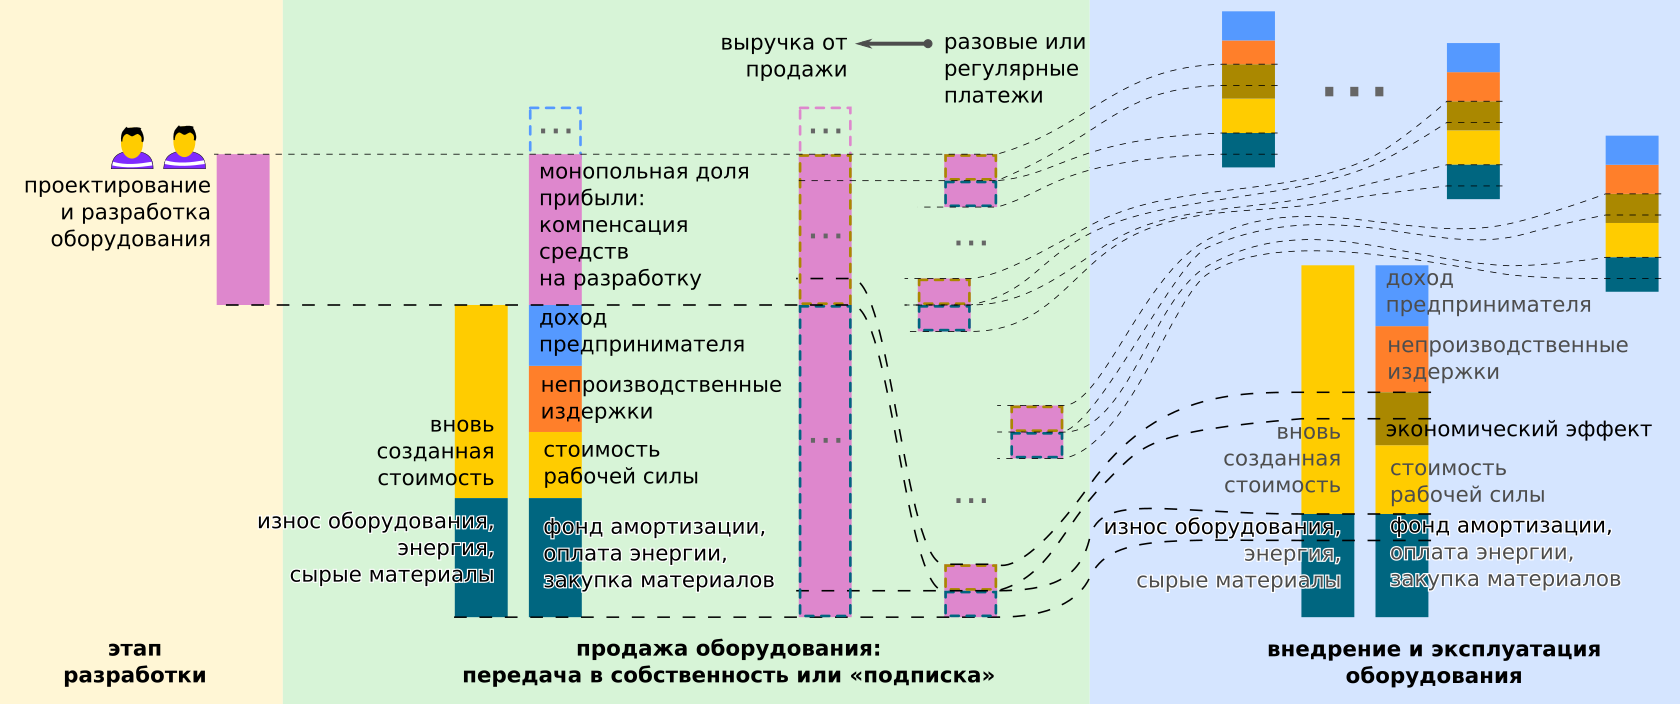
\includegraphics[width=0.95\textwidth]{model-eco-effect-monopoly}
    \caption{Компенсация расходов на разработку производственного оборудования суммой долей экономических эффектов, реализованных внедрившими оборудование потребителями}
    \label{fig:model_eco_effect_monopoly}
\end{figure}

В том случае, если оборудование заметно повышает производительность труда, потребитель вполне может согласиться на относительно завышенную цену, т.~к. он сможет компенсировать её частью экономического эффекта, который реализует результатом внедрения оборудования в собственный процесс производства.

С точки зрения разработчика-производителя, цена его продукта разбивается на две основные части: базовая производственная и добавочная монопольная. Базовая производственная часть составит издержки производства плюс средняя норма прибыли, как в случае с любым материальным продуктом, в т.~ч. аппаратно-программной платформой. Эта часть цены обеспечит нормальное цикличное воспроизводство продукта, при этом не будет учитывать издержки на его разработку. Монопольная часть составит добавочную долю цены сверх базовой. Размер добавочной монопольной части цены может быть рассчитан по схеме, аналогичной модели продажи интеллектуального продукта, к примеру, по модели продажи лицензий на программное обеспечение \cite{businessModels}: все вместе взятые добавочные доли цен проданных продуктов должны, как минимум, компенсировать предварительные издержки на интеллектуальную разработку этих продуктов. С той разницей, что производитель оборудования не продает интеллектуальную собственность как таковую, потребитель не получает обособленную интеллектуальную собственность, а получает в распоряжение готовый материальный продукт, воплощающий в себе эту интеллектуальную разработку.

Базовая производственная часть цены обусловлена объективными факторами производства и не может быть легко изменена производителем. Добавочную монопольную долю цены производитель может варьировать по своему усмотрению, но при этом опираясь на внешние объективные обстоятельства. Нижняя граница добавочной монопольной доли цены единицы продукта определяется размером исходных издержек на разработку и размером планируемой к выпуску партии устройств: монопольная доля в цене всей партии в конечном итоге должна компенсировать исходные фиксированные издержки на разработку. Чем больше партия, тем меньший размер монопольной доли цены можно установить для каждой единицы продукта. Чем меньше партия, тем большая монопольная наценка будет приходиться на каждую единицу продукта. Максимальный размер партии ограничен капиталом, имеющимся в распоряжении производителя, который он готов вложить в производство, а также количеством потенциальных потребителей оборудования на рынке\footnote{«— Lots of analysts have said that everyone who wants a Peloton already bought one. How big is the TAM, or the total addressable market? — You can’t possibly know what the TAM is. You’re in the middle of inventing the TAM.» \cite{nyTimesPeloton2022}}. Верхняя граница добавочной монопольной доли цены, приходящейся на единицу продукта, будет определяться потребителем — покупателем продукта, который принимает решение, какую максимальную цену с его позиций целесообразно платить.

Потребитель, внедряющий оборудование в производственный процесс, может не знать действительное положение границы между базовой производственной частью и монопольной добавочной частью внутри цены рассматриваемого оборудования. Но для того, чтобы оценить целесообразность покупки, он может взять в качестве расчетной базовой производственной части цену имеющегося в его распоряжении или доступного на рынке оборудования, выполняющего аналогичные функции. В качестве монопольной части — оставшуюся долю цены, — она будет не нулевой в том случае, если рассматриваемое оборудование окажется дороже имеющегося в наличии. После этого рассчитанную таким образом добавочную монопольную долю цены он сможет сравнить с предполагаемым экономическим эффектом от покупки и внедрения в производственный процесс нового оборудования (сокращение расхода энергии и сырых материалов, сокращение затрат нового труда на старое количество продукта или увеличение выпуска продукта при прежних затратах труда). В том случае, если экономический эффект от применения нового оборудования превысит расчетную монопольную долю его цены, покупка оборудования имеет экономический смысл, даже если его рыночная цена окажется выше цены оборудования, имеющегося в наличии. В том случае, если экономический эффект применения нового оборудования окажется ниже расчетной монопольной доли его цены, покупка и внедрение такого оборудования будет экономически не целесообразна.

Таким образом, верхняя граница добавочной монопольной доли цены единицы продукта определена экономическим эффектом, который сможет реализовать у себя его применением потребитель этого оборудования. Общее количество добавочной монопольной прибыли, на которое вообще может претендовать производитель оборудования, ограничено сверху суммой всех экономических эффектов, которые смогут реализовать у себя потребители оборудования все вместе взятые.

\section*{\raggedright{Нишевые монополии на основе патентов}}

Наглядным примером применения патентной системы для компенсации издержек на разработку продукта является индустрия производства лекарств — средств, повышающих производительность в сфере медицинских услуг. Новая формула действующего вещества лекарственного препарата обычно разрабатывается внутри фармацевтической компании, формула патентуется, продолжительность патента в США составляет 20 лет\footnote{«After discovering a new drug, manufacturers typically apply for a 20-year patent.» \cite{drugsMarketExclusivityUsa2017}}. В течение этого срока компания-разработчик проводит испытания, получает одобрение регулятора, выводит новое лекарство на рынок и продаёт его под своим брендом, обычно срок эксклюзивного присутствия на рынке для новых лекарств в США составляет 12-16 лет\footnote{«However, after completing preclinical research and up to seven years of clinical trials, only part of this period remains. <...> In total, most brand-name drug manufacturers have a 12-to-16-year window during which their products are free from competition from lower-cost generics.» \cite{drugsMarketExclusivityUsa2017}}. После истечения этого срока конкурирующие производители получают возможность вывести на рынок свои реализации препарата с тем же самым действующим веществом, но под другими названиями — т.~н. «дженерики». Время разработки дженерика значительно сокращено по сравнению со временем разработки оригинального препарата, т.~к. производителю копии, собственно, не требуется изобретать оригинальную формулу, а также не требуется проходить все те же этапы разработки и испытаний, они получают одобрение регулятора по сокращенной процедуре\footnote{«Generic drugs tend to cost less than their brand-name counterparts because generic drug applicants do not have to repeat animal and clinical (human) studies that were required of the brand-name medicines to demonstrate safety and effectiveness.» \cite{genericDrugsFdaUsa2021}}. Дженерики обычно продаются по гораздо более низким, чем у оригинального препарата, ценам, разница в цене может составлять 80-85\%\footnote{«The reduction in upfront research costs means that, although generic medicines have the same therapeutic effect as their branded counterparts, they are typically sold at substantial discounts, an estimated 80 to 85\% less, compared with the price of the brand-name medicine.» \cite{genericDrugsFdaUsa2021}}. С одной стороны, издержки на их разработку не так велики, с другой, при завершении срока патентной монополии на рынке появляется множество игроков и конкуренция снижает цену\footnote{«When multiple generic companies are approved to market a single product, more competition exists in the marketplace, which typically results in lower prices for patients.» \cite{genericDrugsFdaUsa2021}}\footnote{«Generic drug prices are negatively correlated with the number of generic manufacturers in the market» \cite{patentImpactDrugPrices2018}}, приближая её к необходимым издержкам производства с некоторым уровнем средней прибыли. Таким образом, патентная монополия вместе с дополнительными механизмами контроля рынка со стороны регулятора позволяет разработчику лекарств получать добавочную монопольную\footnote{«Government-granted patents and periods of market and regulatory exclusivity provide manufacturers of brand-name pharmaceuticals with monopolies that protect them against competition from generic drug companies.» \cite{drugsMarketExclusivityUsa2017}} прибыль, доля которой в общей цене продукта составляет до 85\% (отношение монопольной доли к оставшейся части цены в таком случае составит до 566.7\%\footnote{85\% / 15\% × 100 = 566.7\%}), часть её использовать для компенсации первоначальных инвестиций на разработку\footnote{«it may be that the brand-name medicine is still within the period of time when it has exclusive rights to the marketplace, which allows drug companies to recoup their costs for the initial research and marketing of the brand-name or innovator drug» \cite{genericDrugsFdaUsa2021}}, реинвестировать в разработку новых лекарств\footnote{«The [drug] industry spends approximately 15\% of sales on marketing, and 16\% of sales on R\&D. By comparison, about 2\% and 3\% of US GDP are allocated to advertising and R\&D, respectively.» \cite{intellectualPropertyAndMarketing2008}}.

В некоторых случаях разработчик оригинального препарата может оставить прежнюю цену после истечения срока патента\footnote{«Of the six studies that assessed the impact of patent expiration on originator prices <...>, the four studies that focused on the USA concluded that originator prices were rigid and overall did not alter significantly after patent expiry <...>.» \cite{patentImpactDrugPrices2018}} или даже повысить её, чтобы компенсировать падение доходов от потери доли рынка\footnote{«although originator prices may increase when more generic manufacturers appear to compensate for losses in market share» \cite{patentImpactDrugPrices2018}}. Таким образом он продолжит получать монопольную прибыль не смотря на то, что на рынке присутствуют недорогие аналоги. В этом случае, однако, монопольное положение будет обеспечено не патентами, а другими факторами\footnote{«For example, while monopolists have incentives to restrict quantity through higher prices, they may also have different incentives to promote their product through advertising, to provide durability of goods, and to vertically integrate with upstream or downstream firms.» \cite{intellectualPropertyAndMarketing2008}} — к примеру, вложениями в рекламу\footnote{«In this model, monopoly always provides too high a price, but it may provide a higher and more efficient level of advertising. This is consistent with the empirical evidence, which suggests that competitive drug manufacturers invest virtually nothing in marketing.» \cite{intellectualPropertyAndMarketing2008}}. Цены на оригинальный препарат обычно всё равно понижаются в течение восьми лет после истечения патента на 30-80\% в зависимости от страны\footnote{«We estimated significant decline in drug prices after patent expiration, ranging from 30 to 80\% depending on the country eight years after patent expiration.» \cite{lifeAfterPatentDrugPrices2023}}.

Заявка на патент на 3D-печать по технологии послойного наплавления пластика (fused deposit modeling — FDM) была подана Скоттом Крампом — основателем компании Stratasys, — в 1989 году, патент выдан в 1992 \cite{fdmPatentUS5121329}, по патентному праву США истек через 20 лет — в 2009. Первый коммерческий принтер, работающий по технологии FDM, был выпущен компанией в 1996 с ценой около \$50 тыс.\footnote{«The result of the co-development deal with IBM was the 1996 introduction of the Genisys 3-D printer. Priced around \$50,000, it was the first RP machine costing less than \$100,000.» \cite{fundingUniverseStratasysHistory2005}} В 2002 компания представила модель Dimension\footnote{«When introduced in 2002 at \$29,900, the Dimension 3D Printer opened new possibilities for designers <...>, at about half the cost of the next [вероятно, имелось в виду “previous”] lowest-price 3D printer» \cite{stratasysDimension2002}}, которая по технологическому исполнению была близка к современным массовым настольным принтерам\footnote{«The IBM wafer system was replaced by a spool of plastic filament that was fed through a heated rod before reaching the nozzle.» \cite{fundingUniverseStratasysHistory2005}}, при цене \$29900 она стала как самым дешевым принтером FDM, так и вообще самым недорогим 3D-принтером из доступных на рынке\footnote{«Moreover, Stratasys was able to price Dimension at less than \$30,000, the least expensive product in the RP and 3D printing markets.» \cite{fundingUniverseStratasysHistory2005}}. В 2008 линейка принтеров FDM была представлена устройствами в ценовом диапазоне от \$18900\footnote{«The Dimension BST (Breakaway Support Technology) is the lowest-priced office-friendly machine of its kind. Priced at \$18,900, the Dimension BST represents a major price breakthrough, powered by leading Stratasys technology.» \cite{stratasysDimensionBst2008}} до \$32900\footnote{«Priced at \$32,900, the [Dimension] Elite features an 8 x 8 x 12-inch build envelope and uses a new, stronger ABS material, ABSplus.» \cite{stratasysElite2008}}. В 2009 Stratasys представила очередной самый дешевый в своей линейке принтер uPrint с ценой \$14900\footnote{«The Dimension 3D Printing Group <...> today [26 января 2009] launched the uPrint Personal 3D Printer (priced at \$14,900 USD) at the annual Dimension reseller conference in Anaheim, Calif.» \cite{stratasysUPrintRelease2009}}. В 2012 году компания выпустила 3D-принтер Mojo по цене \$9900, представленный как персональный\footnote{«Just a few minutes ago [8 мая 2012], Stratasys announced a brand new product in the personal-class called Mojo. <...> For \$9,900, you get everything you need to build and post-process parts. As far as I know, this is the first time that any company has published a price for a 3D printer and the peripherals.» \cite{engineeringStratasysMojo2012}}.

В 2004 году было впервые объявлено о начале работы над проектом RepRap — персональным 3D-принтером FFF (fused filament fabrication, то же, что FDM) с открытыми чертежами и открытым исходным кодом программной реализации управляющих алгоритмов. Ключевой целью проекта была поставлена задача не просто получить открытую реализацию известной технологии, но сделать такое устройство, которое могло бы самостоятельно изготовить максимальное количество собственных узлов. Достижение этой цели не просто избавляло внешние команды, желавшие воспроизвести конструкцию самостоятельно, от необходимости предварительной разработки, но сокращало время на изучение технической документации и поиск ресурсов для создания собственной копии устройства. В 2008 авторы проекта впервые представили модель, которая могла напечатать собственные детали из пластика\footnote{Dr. Adrian Bowyer: «I had the idea for RepRap in 2004, and it first appeared publicly on Bath University’s website in the February of that year. The 10th anniversary this [2018] year is the important one though – it’s the anniversary of the first RepRap making another RepRap: as close as a machine can come to giving birth and so having a birthday.» \cite{rrAnniversaryInterviewAdrianBowyer2018}}. На рынке стали появляться любительские и коммерческие реализации принтеров, которые брали за основу материалы проекта RepRap\footnote{«Mendel <...> used fewer parts and was much simpler to assemble. The release coincided with some stable software and better extrusion techniques and the success with the community was immediate – all of a sudden RepRap’s started popping up everywhere. I was late on my thesis deadline, but RepRap got the mechanics it need to… well… replicate. And it did.» \cite{rrAnniversaryIntervieEdSells2018}}, их авторы продавали отдельные детали\footnote{«From 2010 to 2012 I printed thousands of sets of Mendel and Prusa parts and sold them on eBay. I also supplied some kit sellers, including Adrian.» \cite{rrAnniversaryIntervieChrisPalmer2018}}, функциональные узлы, наборы для сборки и, в дальнейшем, собранные принтеры. Реализация механической части — корпус, кинематика, элементная база, — дорабатывалась\footnote{«В то время только-только начинали появляться opensource настольные 3D-принтеры, доступные широкому кругу людей. <...> Работа над проектом по производству устройств для 3D-печати началась в 2011 году. Через год была создана первая модель наших настольных 3D-принтеров, PICASO 3D Builder, который поступил в продажу в начале 2013 года.» \cite{3dExpoPicaso3D2014}} или полностью заменялась\footnote{«В начале 2014 мы выпустили новый принтер PICASO 3D Designer. PICASO 3D Designer является полностью самостоятельной разработкой с несколькими запатентованными технологиями и кардинально отличается от принтеров предыдущего поколения PICASO 3D.» \cite{3dExpoPicaso3D2014}} от проекта к проекту. Программные прошивки с открытым исходным кодом такие, как Marlin, с точечными доработками или простыми предварительными настройками без доработок использовались в множестве проектов — открытых и проприетарных\footnote{«RepRap firmware, and Marlin in particular, has been huge. Just like GNU/Linux transparently powering everything from ATMs to cable boxes, Marlin has been widely adopted by FFF 3D printer OEMs and is now running on countless 3D printers around the world, and most users have absolutely no idea that it’s a collaborative Free Software project that’s been evolving for years.» \cite{rrAnniversaryInterviewBenMalouf2018}}\footnote{«Right now every vendor maintains their own fork of the one or other Open Source firmware. Based on my experience these forks rarely see bug fixes, improvements or features merged from the upstream versions of those firmwares.» \cite{rrAnniversaryInterviewGinaHaubge2018}}, — даже если они имели значительные внешние и внутренние отличия в механике\footnote{«No one agrees on what the definitive hardware design should look like. Firmware is all over the map. Software too. There is little common ground and so very little that is neutral territory between two open source companies.» \cite{rrAnniversaryInterviewBrookDrumm2018}}. В связке с типовыми электронными платами с открытыми чертежами такими, как RAMPS, они еще ниже опускали порог выхода на рынок для новых разработчиков и производителей. По данным сайта RepRap по состоянию на конец 2012 года в активной разработке находилось 9 прошивок с открытым исходным кодом \cite{rrListOfFirmware2012} (некоторые из них являлись ответвлениями других проектов из этого же списка). В базе данных RepRap Family Tree собрано 220 моделей принтеров, работавших по технологии FFF, созданных с 2006 по 2013 годы \cite{rrFamilyTree2013}. Для значительной части проектов из списка отслеживается их прямое происхождение от проектов семейства RepRap, кратный рост количества новых моделей начинается в 2009-2010 годы.

Первая коммерческая компания, использовавшая разработки проекта RepRap, — MakerBot, — была основана в 2009 году, в этом же году она выпустила в продажу первый продукт — набор для самостоятельной сборки 3D-принтера CupCake CNC \cite{thingiverseCupCakeCnc2009} по цене \$750 за экземпляр\footnote{«In January 2009 the trio founded MakerBot <...> to sell the CupCake as a kit for people to assemble. By the spring, MakerBot was shipping CupCake kits for \$750 apiece.» \cite{wiredMakerbot2016}}\footnote{«MakerBot was the first company based on RepRap.» \cite{rrOfficialHistory2016}}. Новые коммерческие разработчики-производители также начали игру на массовом рынке\footnote{«Over the past decade we’ve seen small businesses (Lulzbot, Prusa, Printrbot etc) push 3D printing technology into the hands of everyone, and in doing so the technology has been exposed to some intense competition.» \cite{rrAnniversaryIntervieEdSells2018}}. Новый рынок обладал высокой степенью конкуренции\footnote{«It was very hard to predict future demand because it fluctuates wildly with currency changes and, with a new 3D printer coming out nearly every day, there is a risk sales could suddenly dry up if a better cheaper kit emerged.» \cite{rrChrisPalmerEndGame2015}}, что приводило к максимальному удешевлению конструкций, с одной стороны, и к улучшению технологии исправлением тех или иных распространенных проблем в каждой новой модели — с другой. Цена некоторых устройств доходила до \$200 (по крайней мере, продаваемых в виде набора \cite{geekdadOneUp2014}), но приближение цены к этой планке уже требовало компромиссов в конструкции, качестве используемых материалов, наборе полезных пользовательских функций и надежности эксплуатации\footnote{«I mean, it’s a \$200 3D printer <...> If you’re expecting to match the speed and quality of a (current) \$3000 3DP, you’re going to be disappointed.» \cite{geekdadOneUp2014}}.

Продажная цена модели Buildatron 2 в виде набора для самостоятельной сборки (т.~е. в разобранном виде) в 2012 году составляла \$1600, цена этой же модели в собранном виде (сборка производится на стороне производителя) составляла \$2500\footnote{«If you're thinking that there may be a 3D printer in your immediate future, the Buildatron 2 (\$1,599 direct in kit form or \$2,500 assembled), is good place to start.» \cite{pcmagBuildatron2012}}. Таким образом, часть цены готового устройства, определяемая необходимым для сборки конструкции трудом, для этой модели составляла \$900\footnote{\$2500 - \$1600 = \$900}, т.~е. 36\% от цены готового устройства\footnote{\$900 / \$2500 × 100 = 36\%}, доля стоимости компонент — 64\%. Цена одной из наиболее успешных персональных моделей 3D-принтера с достаточно простой минималистичной конструкцией — Prusa, — в 2024 году в разобранном виде составляла \$800, в собранном — \$1100\footnote{3D-принтер Original Prusa MK4S 3D Printer, цены по состоянию на 2024 на сайте производителя: «Kit: \$799», «Assembled: \$1099» \cite{prusa2024}}. Часть стоимости, присоединенная сборкой, в этом случае составила \$300\footnote{\$1100 - \$800 = \$300}, её соотношение с долей стоимости компонент в цене собранного устройства составило 27\%\footnote{\$300 / \$1100 × 100 = 27.3\%} к 73\%. Таким образом, для разных моделей доля стоимости, созданной трудом по сборке финальной конструкции, может варьироваться, но во всех случаях она составляет заметную в относительном выражении величину, в абсолютном выражении сопоставимую с уже достигнутым минимумом цены устройств в \$200 или превышающую его. На этих основаниях можно заключить, что линия по удешевлению на текущем витке развития технологий производства достигла предела. Реализация новых возможностей, действительно улучшающих потребительные свойства устройств, требовала добавления к минималистичной конструкции дополнительных функциональных узлов и деталей, что могло только удорожить как стоимость набора компонент, так и сложность и стоимость труда по сборке\footnote{«Currently RepRap machines need far too much human effort to replicate to spread exponentially as Adrian envisaged.» \cite{rrAnniversaryIntervieChrisPalmer2018}}.

Часть игроков отказалась от участия в «гонке за дешевизной»\footnote{«But I believe the race to the bottom (price), won largely by Chinese knock-offs, was a loss for idealists, purists, and even capitalists.» \cite{rrAnniversaryInterviewBrookDrumm2018}} и сделала упор на создании моделей с улучшенными конструкциями с более высокими надежностью, качеством и скоростью печати. Достигнув нижнего предела, цены опять пошли вверх до нескольких тысяч долларов за устройство. Однако в этом случае рост был обусловлен не монополией, а функциональными улучшениями продуктов при объективных ограничениях современных технологий производства\footnote{«They [3D printers] need to be self assembling because most people are not interested in putting something together themselves.» \cite{rrAnniversaryIntervieChrisPalmer2018}}. Эксплуатационные свойства таких моделей стали пригодны для применения в инженерном и производственном бизнесе\footnote{«Volkswagen has announced that, in 2016, the factory made an annual saving of \$160,000 using FDM desktop 3D printers – reducing typical production costs by over 90\% and taking 95\% less time on tool development. Remarkably the 3D printers are not the industrial machines with price tags of \$100,000 upwards, but desktop 3D printers from Ultimaker.» \cite{3dprintingindustryVolkswagenUltimaker2017}}, т.~е. для решения задач, на которые изначально была нацелена Stratasys. К примеру, у компании Ultimaker линейка принтеров, нацеленных на промышленный сектор (изначально разработана MakerBot), в 2024 году представлена моделями с ценами от \$4999 (Method 3D Printer) до \$13999 (Method XL 3D Printer) \cite{ultimakerMethod2024}, что всё равно в 2-3 раза ниже, чем цены на линейку промышленных моделей Stratasys времён действия патентной монополии. Если исходить из того, что промышленные 3D-принтеры начального уровня в линейках Ultimaker (Method 3D Printer, \$4999, выпущен в 2018\footnote{«We thought differently. We thought, what are the minimum specifications that you want to have in the professional market, and then, what is the lowest price you can get?» \cite{3dprintingindustryMakerBotMethod2018}}, цена по состоянию на 2024) и Stratasys (Dimension BST, \$18900, 2008) имеют примерно одинаковые потребительные свойства и являются взаимозаменяемыми на некотором классе типичных для своего сегмента задач\footnote{«However, printer companies focused on prototyping materials and applications will find their profit margins challenged by falling prices and rising competition, particularly from hundreds of suppliers of sub-\$3,000 desktop printers with capabilities comparable to the \$20,000 prototyping printers of just 5 to 10 years ago.» \cite{nstiLuxHow3dPrintingAddsUp2014}}, в цене Stratasys Dimension BST можно выделить монопольную долю прибыли, она составит \$13901\footnote{\$18900 - \$4999 = \$13901}, или 278\%\footnote{\$13901 / \$4999 × 100 = 278\%} от оставшейся немонопольной части цены.

По оценке Wohlers Associates рынок 3D-печати, — включая материалы для печати, напечатанные изделия и сами принтеры, применяющие любые технологии 3D-печати, не только FDM/FFF, — достиг \$2.2 млрд. в 2012 году, удвоившись с \$1 млрд. за предшествующие пять лет\footnote{«The market for 3D printing in 2012, consisting of all products and services worldwide, grew 28.6\% (CAGR) to \$2.204 billion. <...> It took the 3D printing industry 20 years to reach \$1 billion in size. In five additional years, the industry generated its second \$1 billion.» \cite{wohlersReport2013}}. В исследовании Lux Research в 2014 году всего четыре компании были отмечены как доминирующие на рынке, их общая доля составляла 31\% рынка\footnote{«On the Lux Innovation Grid, only four printer companies placed in the “Dominant” category based on technical and business scores: 3D Systems, Stratasys, EOS, and Arcam. The four hold a combined 31 percent printer market share.» \cite{luxResearchHow3dPrintingAddsUp2014}}, из чего можно заключить, что значительную часть (69\%) рынка занимало большое количество средних и мелких игроков, не являвшихся монополистами. Рынок персональных 3D-принтеров (устройств с ценой до \$5 тыс. по классификации Wohlers), взятый отдельно, по данным Wohlers при этом рос в среднем на 346\% каждый год с 2008 по 2011, в 2012, однако, темпы его роста существенно замедлились\footnote{«Growth of the low-cost (under \$5,000) “personal” 3D printer market segment averaged 346\% each year from 2008 through 2011. In 2012, the increase cooled significantly to an estimated 46.3\%» \cite{wohlersReport2013}}. По оценке Gartner в 2013 году технологии персональной 3D-печати находились на пике внимания и ожиданий\footnote{«At the Peak: Consumer 3D Printing» \cite{gartnerHype2013}}, в популярных изданиях они зачастую преподносились как появившиеся недавно\footnote{«Founded in 2009, the company shot to prominence during the rise of 3D printing, a new technology that allows ordinary consumers and businesses to build polymer-based products in their homes or places of work.» \cite{cnetMakerBot2UsSchools2013}}. Промышленная 3D-печать в то же время по классификации Gartner вступала в стадию зрелости\footnote{«Climbing the Slope: Enterprise 3D Printing» \cite{gartnerHype2013}}. В 2022 году общий рынок 3D-печати достиг \$18 млрд. (Wohlers) \cite{wohlersReport2023}, рынок персональной 3D-печати в 2023 — \$2.11 млрд. (Expert Market Research)\footnote{«In 2023, the market reached an approximate value of USD 2.11 billion.» \cite{expertMarketResearchPersonal3dp2023}}. Т.~е. спустя десять лет рынок персональной 3D-печати достиг размера, который в 2012 году имел весь рынок 3D-печати целиком.

Таким образом, истечение срока патентной монополии, с одной стороны, открыло рынок для множества производителей, конкуренция между которыми опустила цены до минимальных границ, определяемых издержками на производство. С другой стороны, свободно доступная работающая реализация технологии, в частности, программная прошивка, в значительной степени опустила планку выхода на открывшийся рынок для новых производителей\footnote{«Right now [2018], several of the largest 3D printer manufacturers (by unit and/or by revenue) are, or at least began as, Open Source companies.» \cite{rrAnniversaryInterviewBenMalouf2018}}, т.~к. их предварительные издержки на разработку, а также необходимое время разработки до выхода на рынок оказались относительно невелики. Всё вместе это привело, во-первых, к появлению нового класса устройств — персональных 3D-принтеров, — и вместе с ними полностью нового рынка персональной потребительской 3D-печати\footnote{«As well as an immediate effort towards self-replication, we opened up a multi-billion dollar industry now known as 3D printing.» \cite{rrAnniversaryIntervieEdSells2018}}\footnote{«RepRap is what turned 3D printing from a walled garden technology into a mass market phenomenon, available and affordable for hobbyists. Without it, 3D printing would probably still be a technology unavailable to anyone but companies capable of affording the expensive commercial machines and we would have seen a lot less innovation in the market.» \cite{rrAnniversaryInterviewGinaHaubge2018}}\footnote{«The 3D printing industry as we know it today owes it’s existence to the RepRap project. That is not to say RepRap didn’t have forebearers, obviously it did, but prior to RepRap most people hadn’t even heard of 3D printing, let alone had they seen or used a 3D printer. That has changed significantly in the last 10 years. Regardless of whether or not you think 3D printers belong in the average home, the hype centered around that concept fundamentally changed the industry and fueled its growth.» \cite{rrAnniversaryInterviewBenMalouf2018}}. Во-вторых, к тому, что цены на существующем сложившемся рынке промышленной 3D-печати были опущены в несколько раз.

\section*{\raggedright{Нишевые монополии на основе сокрытия деятельности и технологий}}

Удержание технологий в секрете, как и патенты, ограничивает возможности конкурентов применять технологию в собственных продуктах, поэтому является инструментом создания нишевой технологической монополии. В некоторых случаях разработчик технологического продукта может удерживать в секрете не только технологию, но и сам факт своей деятельности по распространению продукта среди потребителей, т.~е. действовать в т.~н. режиме «стелс».

Информацию о компаниях, действующих на рынке в скрытном режиме, в открытых источниках найти не всегда легко. Однако, из особенности этой стратегии можно заключить, что в абсолютном количестве клиентов у таких производителей будет относительно немного, т.~к. инструменты широкого маркетинга такой стратегии не соответствуют. Таким образом, издержки на разработку внедряемого продукта должно окупить небольшое количество потребителей. Стоимость разработки в таком случае должна быть относительно невелика или в точках внедрения достаточно большим должен быть экономический эффект. Реализацию большого экономического эффекта, обеспечиваемого масштабом внедрения, можно ожидать у крупных потребителей. При небольшом количестве клиентов такая модель окажется близка к модели внутрикорпоративной разработки, при которой значительную долю разработки оплачивает один игрок (но здесь игроков может быть несколько).

В тематической публицистике под компаниями, работающими в режиме «стелс», обычно имеют в виду компании, находящиеся на стадии разработки продукта, скрывающие эту разработку\footnote{«Operating in stealth mode also can help protect intellectual property until launch» \cite{startupsStealth2013}}. Герман Саймон в книге «Скрытые чемпионы XXI-го века» («Hidden Champions of the Twenty-First Century») 2009 года исследовал действующие зрелые компании, продающие собственные готовые высокотехнологичные продукты\footnote{«Surprisingly, about 70\% (exactly 69.7\%) claim the technological development stage is mature, meaning the typical hidden champions’ products are high-tech, but no longer in the experimental phase.» \cite{hiddenChampions2009}}, которые если не скрывают, то, по крайней мере, специально не афишируют сам факт своего присутствия на рынке. Ранее для таких компаний он же придумал и ввел в оборот термин «скрытые чемпионы» (\textit{hidden champions}). По оценке Саймона на момент публикации книги скрытые чемпионы занимали 33.0\% мирового рынка и 38.4\% рынка Европы\footnote{«The hidden champions’ average absolute market share is 33.0\% for the world market and 38.4\% for Europe. It is astonishing that both figureshave increased over the last ten years.» \cite{hiddenChampions2009}}. Фактическое отсутствие широкой известности отчасти объясняется тем, что компании такого рода часто являются поставщиками для других компаний — производителей продукта для конечного потребителя, — поэтому в массовой рекламе нет нужды\footnote{«Why have these outstanding companies, all of which occupy leading positions in their markets worldwide, remained hidden? There are many reasons, but the most obvious is that a large number of the products offered by hidden champions go unnoticed by consumers. Many of these companies operate in the “hinterland” of the value chain, supplying machinery, components or processes that are no longer discernable in the final productor service.» \cite{hiddenChampions2009}}\footnote{«Keeping a low profile in the public eye, the media and the research sector offers advantages that should not be underestimated: it helps companies to focus on their business. Jim Collins makes a telling distinction between “show horses” and “plough horses.” The plough horses do not put much time or effort into grooming their public image, so they save time and energy to concentrate on their true purpose: conducting good business.» \cite{hiddenChampions2009}}. При этом в профессиональном сообществе среди потенциальных потребителей такие специализированные производители хорошо известны\footnote{«Hidden champions may be little known to the general public, but they are very well known and have an excellent reputation among their direct customers.» \cite{hiddenChampions2009}}. Для привлечения новых клиентов подавляющее большинство скрытых чемпионов предпочитают прямые продажи широкой рекламе\footnote{«82.6\% of the hidden champions say they engage in direct sales while 29.5\% sell via intermediaries. <...> Approximately 70\% of the hidden champions only sell directly» \cite{hiddenChampions2009}}. Однако во многих случаях скрытность или ограниченная известность является осознанной целенаправленной политикой, целью которой является создание условий, при которых внимание потенциальных конкурентов не будет привлечено, т.~е., в конечном итоге, — сохранение монопольного положения в удачно занятой нише\footnote{«Another reason why hidden champions remain concealed is that they avoid drawing attention to themselves. According to the CEO of theworld’s leading manufacturer of textile needles, “every unwanted public mention of our company counteracts our efforts to stay unknown.”» \cite{hiddenChampions2009}}\footnote{«The CEO of the world’s number one manufacturer of a key shock absorption component remarked to me, “We want neither our competitors nor our customers to know our true marketshare.” In a similar discussion, the CEO of a service provider stated, “We have cherished our anonymity for years and feel very comfortable about it. Nobody has noticed our niche.”» \cite{hiddenChampions2009}}\footnote{«A lack of transparency can have its advantages. Albert Blum, founder of ABS Pumps, once told me, “If you don’t know the size of your market and your market share, you need not fear the Japanese.” I will not attempt to answer as to whether this statement also applies to the Chinese. However, my impression is that, in contrast to the Japanese, the Chinese also venture into markets for which they cannot obtain reliable statistics.» \cite{hiddenChampions2009}}.

Кроме скрытности в медийном пространстве, скрытые чемпионы полагаются на ограничение доступа к технологиям для сохранения исключительности позиций. Обычно такие компании уделяют большое внимание технологиям и выделяют на них ресурсов в среднем значительно больше, чем многие другие компании, реинвестируя в исследования и разработки 6-9\% выручки\footnote{«These companies spend 5.9\% of revenues on research and development (i.e., twice as much as the average innovators in the German Economic Institute study and almost 50\% more than the top 1,000 R\&D companies in the world). For one fifth of the hidden champions, the R\&D intensity actually exceeds 9\%, more than three times the typical figure for German companies.» \cite{hiddenChampions2009}}. Новые разработки нужны, во-первых, для того, чтобы потребительные свойства продукта превосходили свойства ближайших аналогов, создавая исключительность в глазах потребителя. Во-вторых, чтобы производительность труда при производстве продукта внутри компании находилась на приемлемом уровне. Хотя компании достаточно активно патентуют свои разработки\footnote{«On average, patent intensity is more than five times higher for the hidden champions. The number of patent applications per 1,000 employees is 5.8 for large corporations and 30.6 for the hidden champions. R\&D expenditure per patent applicationis \$724,730 for the selected hidden champions, but \$3.55 million for the large corporations — around five times higher. The value of these patents is unknown, but the assumption that the patents of large corporations have a higher value is not confirmed. According to the study, “larger companies do not have more valuable patents, as might be assumed.”» \cite{hiddenChampions2009}}, для ограничения доступа к технологиям они часто полагаются на сокрытие технологий, а не на патенты\footnote{«According to a study by the European Patent Office, two thirds of the small and midsize companies that actively engage in research and development do not protect their innovations through patents. Smaller companies are often deterred by the red tape, costs, or time required to obtain patents. Further reasons for the reticence are doubts about beingable to enforce patents against large competitors or in legal proceedings abroad, or about disclosing expertise. “We do not apply for patents because we do not have the people to do it and we hate the bureaucracy,” explains Klaus Grohmann of Grohmann Engineering, a highly innovative company. “In any case, innovation in our sector is very fast compared with how long it takes to obtain a patent.”» \cite{hiddenChampions2009}}. Если конечный продукт, попадающий в руки потребителей, скрыть не всегда легко, сокрытию подлежат внутренние технологии производства такого продукта, в том числе, например, специализированное оборудование, которые было создано внутри компании исключительно для реализации нужд некоторых внутренних технологических процессов\footnote{«The hidden champions’ preference for doing things themselves often goes further and includes earlier steps in the value chain. As mentioned in Braun’s quote, many of these companies have their own mechanical engineering departments. At Hoppe, one of the market leaders for door and window fittings, I was told, “Around 10\% of our workforce build our own machinery which we keep very secret. We develop and produce our own machines and we don’t sell them to others. These machines encompass our core competencies.”» \cite{hiddenChampions2009}}.

Хотя их внутренняя производительность может быть выше, чем у ближайших конкурентов, скрытые чемпионы, как правило, не используют её для укрепления позиций за счет понижения цены\footnote{«Profits can only be earned with low prices if a company can manufacture at lower costs than the competition over a sustained period of time.» \cite{hiddenChampions2009}}, а, напротив, продают продукт дороже, чем конкуренты\footnote{«With few exceptions, the hidden champions do not gain their market shares with low or aggressive prices, but with superior performance. They “earn” their market leadership by being the best in technology, innovation, quality, reputation, and so forth.» \cite{hiddenChampions2009}}, что также говорит о том, что они реализуют возможность получения монопольной доли прибыли. Скрытые чемпионы ориентируются на узкие и сверхузкие ниши (\textit{суперниши}), в рамках которых они производят уникальный востребованный продукт, занимая при этом доминирующее положение в нише\footnote{«The hidden champions usually focus on narrow markets. Many of them do not feel restricted by customary market boundaries, but define their markets autonomously as part of their strategy. In doing so, hidden champions often achieve high market shares with sometimes monopolistic positions; thereby establishing effective barriers to entry.» \cite{hiddenChampions2009}}\footnote{«Numerous hidden champions take their market definitions even further and specialize in extremely narrow niches. Some “create” their markets so that there are no real competitors and they have 100\% market share. The list of such companies adds up to hundreds.» \cite{hiddenChampions2009}}. Востребованность является следствием того, что продукт, применяемый внутри технологических процессов потребителя, создает для потребителя некоторый экономический эффект, без этого продукта его деятельность была бы организована заметно менее эффективно вплоть до исчезновения целесообразности ведения самой деятельности\footnote{«More than 70\% of the customers depend on a product offered by the hidden champion. However, only 20\% of the hidden champions say that their customers are completely dependent on them» \cite{hiddenChampions2009}}. Уникальность, т.~е. отсутствие конкурентов или подавляющее доминирование над ними\footnote{«The typical hidden champion faces a limited number of competitors. On average (median), the hidden champions have six serious competitors on the world market. Almost 60\% (exactly 59.8\%) have fewer than ten competitors worldwide and only 12.8\% have more than 20 competitors.» \cite{hiddenChampions2009}}, даёт возможность производителю претендовать на долю этого экономического эффекта, реализуемого на стороне потребителя, через добавление в цену монопольной доли прибыли.

По оценке Германа Саймона, цена продукта скрытого чемпиона обычно на 10-15\% выше средней рыночной цены аналогичных продуктов, в некоторых случаях еще выше\footnote{«In most cases, their superior performance permits them to charge significantly higher prices. In my experience and as a result of many conversations, I estimate that the typical price premium of a hidden champion versus the market average is 10\%–15\%, sometimes even higher.» \cite{hiddenChampions2009}}, эту премиальную часть цены можно рассматривать как монопольную долю прибыли. При этом она ограничена сверху экономическим эффектом, который сможет реализовать на своей стороне потребитель продукта при помощи покупки\footnote{«The customer is prepared to pay a reasonable premium for higher quality and performance. However, there are limits to the willingness to pay, so the costs must always be kept under control.» \cite{hiddenChampions2009}}\footnote{«The opposite is probably true: they do not fully exploit their pricing power. There is considerable potential for improved quantification of the value to customer (which should always be the basis for price setting) and in a refined price differentiation.» \cite{hiddenChampions2009}}, превышение этой границы сделает покупку экономически нецелесообразной\footnote{«The aim is not to make costs and prices a strategic competitive advantage, but to prevent a company from pricing itself out of the market.» \cite{hiddenChampions2009}}. Еще одна особенность существенной части скрытых чемпионов заключается в том, что количество прямых потребителей их продуктов, действительно, невелико\footnote{«Just over 10\% of the hidden champions generate more than half their total revenues from the five largest customers. The printing technology supplier Technotrans, for example, earns 60\% of its revenues from the three leading printing press manufacturers Heidelberg, Manroland, and Koenig \& Bauer. This means high dependence on very few customers, although this dependence is not necessarily one-sided. <...> The second group, where 20\%–50\% of the total revenues are generated with the five leading customers, is significantly larger, at 28\%.» \cite{hiddenChampions2009}}. Деятельность скрытых чемпионов и их клиентов не редко глубоко интегрированы друг в друга\footnote{«The hidden champions’ relationships with their customers are close and interactive. The main reason is that, in general, they offer complex product and service programs, often even systems solutions. Such programs cannot be sold off the peg, but require detailed consultation processes.» \cite{hiddenChampions2009}}. Если производитель продукта хорошо знает, каким образом будет внедрен его продукт на конкретном предприятии, он сможет достаточно близко оценить производный экономический эффект, и, опираясь на эту оценку, включить в цену часть этого эффекта, получив таким образом монопольную долю прибыли. Скрытые чемпионы часто могут позволить себе индивидуальный подход как в развитии продукта, ориентируясь на нужды ключевых клиентов, так и в установлении индивидуальной для каждого клиента цены\footnote{«The pricing processes also deserve greater attention. As most hidden champions are active in business-to-business markets, actual transaction prices are almost always negotiated.» \cite{hiddenChampions2009}}, задающей границу распределения экономического эффекта между покупателем и продавцом\footnote{«However, the balance between value delivery and value extraction proves delicate.» \cite{hiddenChampions2009}}.

\section*{\raggedright{Закрытое программное обеспечение как инструмент сегментирования рынка аппаратных продуктов}}

Компании, производящие продукт для массового рынка, могут скрывать свои внутренние технологические процессы. Для защиты от копирования готового продукта они вынуждены полагаться на патенты. В случае с аппаратно"=программной платформой программная составляющая устройства играет важную роль в его потребительных свойствах. Для того, чтобы скопировать успешный продукт, потенциальный конкурент должен повторить не только корпус, механику и электронику, но также воспроизвести программные управляющие алгоритмы оригинала. Управляющие программные алгоритмы обычно пишут на языках высокого уровня, в тело устройства они входят в виде машинного кода — двоичной программной прошивки. Даже в том случае, если двоичный машинный код удастся извлечь из памяти устройства, оригинальный код на языке высокого уровня из него обычно невозможно восстановить. В отдельных случаях его можно использовать с точечными правками или без изменений «как есть» в устройстве, являющемся максимально близким клоном с полностью совместимой аппаратной платформой оригинала, но не для развития собственного продукта на базе успешного существующего. Существуют технологии, которые позволяют сделать невозможной или существенно затруднить процедуру извлечения даже двоичной программной прошивки\footnote{«Secure and encrypted boot helps ensure that the executing software is authentic and unreadable.» \cite{timesysIotDevProtection2022}}. Таким образом, применение закрытого проприетарного программного кода в аппаратно-программном продукте является фактором ограничения конкуренции, приближающим производителя, применяющего такой код, к положению нишевого технологического монополиста.

В некоторых случаях программная логика используется не для реализации полезных функций устройства, а для искусственного сегментирования рынка в линейке продуктов производителя, т.~е., в конечном итоге, для получения монопольной доли прибыли, по крайней мере, для части своих продуктов.

Одна из особенностей технологического процесса производства микропроцессоров, по крайней мере, в 1990 — 2000 годы заключалась в том, что качество чипов, размещенных на одной и той же заготовке — диске кремния («вафле»), — т.~е. производимых в рамках одного и того же производственного цикла, могло существенно отличаться: некоторые из них работали стабильно на целевой тактовой частоте генератора импульсов, другие при тех же обстоятельствах показывали нестабильную работу, но могли при этом достаточно надежно выполнять свои функции на более низких частотах. При таких обстоятельствах производители микрочипов — на тот момент лидеры рынка Intel и AMD, — имели возможность не списывать менее стабильные экземпляры чипов в брак, а выводить их на рынок как отдельную «лоу-энд» версию чипа, имеющего ту же внутреннюю микроархитектуру, что и удачные («хай-энд») экземпляры, только с более низкой штатной скоростью работы, продавая их, соответственно, по более низкой по сравнению с более быстрыми экземплярами цене, разделив таким образом рынок чипов на «хай-энд» и «лоу-энд» в рамках одного и того же поколения микроархитектуры и технологического процесса производства.

Таким образом, усредненные издержки производства в пересчете на отдельный чип как в случае хай-энд, так и в случае лоу-энд версии были равны, но на рынке они были представлены под разными маркетинговыми именами и по разной цене, т.~к. в противном случае потребители покупали бы только более производительный вариант чипов, продукты одного и того же производителя составляли бы друг другу конкуренцию. Вместе с тем, процесс тестирования и сортировки чипов на высокопроизводительные и менее производительные был выстроен таким образом, что среди чипов, отправленных в группу лоу-энд, регулярно оказывалось некоторое количество высококачественных чипов, которые могли работать в полную силу. В сообществе пользователей вычислительной техники получила распространение теория, по которой производители также могли целенаправленно отправлять некоторое количество известных хай-энд чипов в сегмент лоу-энд, например, в том случае, если бы расчетный спрос на готовые хай-энд процессоры оказался бы недостаточным, но их всё еще можно было продать в лоу-энд варианте. Так или иначе, исследователи и энтузиасты заметили, что при помощи некоторых технических ухищрений некоторые компьютеры с чипами, купленными как недорогой лоу-энд вариант процессора, можно запускать на повышенной тактовой частоте, получая такую же производительность, как на компьютерах с установленными изначально дорогими хай-энд чипами.

Авторы книги «Книга оверклокинга — раскрой потенциал своего ПК» («The Book of Overclocking — Tweak Your PC to Unleash Its Power») \cite{theBookOfOverclocking2003} приводят в пример лоу-энд вариант чипа Intel Pentium 4 с штатной частотой 2000 МГц с подтвержденным потенциалом разгона до 2600 МГц, а также хай-энд вариант чипа того же поколения Intel Pentium 4 с штатной частотой 2600 MHz. Средняя рыночная цена первого чипа по данным на 2002 год составляла \$143, второго — \$378. Если принять цену лоу-энд варианта за базовую производственную цену, определяемую издержками производства и средней нормой прибыли, разница между его ценой и ценой соответствующего хай-энд чипа составит премиальную наценку на базовую цену — монопольную долю прибыли в цене хай-энд чипа. В случае с приведенными моделями Intel Pentium 4 она составит \$235\footnote{\$378 - \$143 = \$235} или 164\%\footnote{\$235 / \$143 × 100 = 164\%} от базовой цены чипа. Аналогичным образом в том же источнике: лоу-энд чип AMD Athlon XP 1600+ @1400 МГц с потенциалом разгона до 1800 МГц со средней ценой \$53 в том же 2002 году и его хай-энд вариант — AMD Athlon XP 2100+ @ 1800 МГц с ценой \$141. Монопольная наценка в этом случае составит \$88\footnote{\$141 - \$53 = \$88} на хай-энд чип, монопольная доля прибыли от базовой производственной цены — 166\%\footnote{\$88 / \$53 × 100 = 166\%}.

Возможность разгона (оверклокинга) недорогого лоу-энд процессора до характеристик хай-энд варианта требовала некоторого уровня везения при покупке, осведомленности, технической подготовленности и инициативы пользователей, поэтому движение оверклокинга не могло полностью поломать модель сегментирования рынка производителей процессоров. Тем не менее, производители чипов в некоторой момент начали применять технические средства для ограничения возможностей оверклокинга своих продуктов. Тактовая частота процессора на персональных компьютерах задавалась в два этапа: кварцевый генератор, размещенный на материнской плате, генерирует колебания на относительно низкой частоте, далее частота колебаний повышается в несколько раз или десятков раз внутри процессорного чипа через специальный умножитель. Таким образом, повысить частоту процессора можно было или снаружи процессора, увеличив частоту колебаний на шине, ведущей от генератора в процессор, или выставив более высокий коэффициент умножителя частоты внутри процессора через его настройки. Вариант с настройкой умножителя был предпочтительнее, т.~к. позволял более гибко задавать целевую частоту процессора, а также не затрагивал прочие устройства, подключенные к шине базового генератора на материнской плате. Производители материнских плат обычно позволяли задавать настройки умножителя через специальные перемычки на плате или интерфейс БИОС в том случае, если это позволял процессор.

Начиная с отдельных моделей и партий в линейке Pentium 2, продолжая полной линейкой Pentium 3, Intel начала блокировать возможность настройки умножителя внутри своих чипов, чем существенно ограничила возможности разгона своих процессоров. AMD тоже блокировала штатный интерфейс изменения настроек умножителя, но энтузиасты заметили, что на них можно было влиять через некоторые элементы, выведенные на внешнюю часть чипа. На рынке появились специальные устройства (т.~н. Gold Finger Devices), которые позволяли менять настройки умножителя в чипе и, таким образом, разгонять процессор. В очередном поколении чипов AMD сменила способ блокировки умножителя, для разблокировки пользователю было достаточно восстановить контактную дорожку на корпусе чипа, например, прочертив её электропроводящим карандашом. Исходная дорожка разрушалась лазером на этапе производства. Позднее AMD отказалась от этой процедуры, т.~к. она удорожала производство и добавляла вероятность повреждения исправного чипа. Многие модели чипов AMD начала выводить на рынок сразу разблокированными: хотя, с одной стороны, это не соответствовало модели сегментирования рынка, с другой стороны, это могло являться дополнительным конкурентным преимуществом в борьбе с главным соперником на рынке — компанией Intel.

Даже в том случае, если качество изделий, производимых массово, не отличается серьезно по целевым свойствам, производители все ещё применяют методы искусственного сегментирования рынка по ценовым категориям\footnote{«But the marketing department will insist on having several options in the line. It’s part of a concept called market segmentation which seeks to tailor products to carefully selected groupings of customers.» \cite{hackdayUnlockableFeatures2017}}, отключая доступные изначально полезные функции у лоу-энд экземпляров линейки. В условиях массового производства обычно дешевле произвести большую партию одинаковых изделий, чем несколько партий меньшего размера немного отличающихся друг от друга изделий. При этом изначальное исключение из конструкции отдельных функций или компонент может не дать существенную экономию при производстве. Проектирование двух различных вариантов устройства с разным набором функций также удорожает этап инженерной разработки устройства\footnote{«hardware developers don’t want to follow several parallel designs through to production» \cite{hackdayUnlockableFeatures2017}}. Таким образом, в некоторых случаях по сумме причин производители предпочитают произвести одну партию идентичных устройств с максимальным набором функций, а затем заблокировать некоторые из них\footnote{«The easiest thing to do is to design with all the bells and whistles and throw some of them overboard for the mid- and low-tier offerings. This is fairly painless to do with software.» \cite{hackdayUnlockableFeatures2017}}, чтобы иметь возможность проводить ценовую политику сегментирования рынка и, в конечном итоге, получать монопольную прибыль\footnote{«Companies look for the biggest margin, and that is going to be high-end equipment where they can differentiate themselves from competitors and where businesses with purchasing power are the customer.» \cite{hackdayUnlockableFeatures2017}}.

Производители осциллографов ограничивают максимальную частоту и блокируют отдельные интерфейсные модули на моделях начального уровня, при этом используют для этих недорогих моделей и полнофункциональных дорогих одну и ту же аппаратную базу\footnote{«More famously, oscilloscopes have been notorious for having crippled features. The Rigol DS1052E was hugely popular on hacker benches because of it’s very approachable price tag. The model shipped with 50 MHz bandwidth but it was discovered that a simple hack turned it into the DS1102E 100 MHz scope. Tektronix has gotten in on this action as well, shipping modules like I2C, CAN, and LIN analyzation on the scope but requiring a hardware key to unlock (these were discovered to have a horribly insecure unlock method). Similar feature barriers are found on Rigol’s new reigning entry-level scope, the DS1054Z, which ships with protocol analyzation modules (among others) that are enabled only for the first 70 hours of scope operation, requiring an additional payment to unlock them.» \cite{hackdayUnlockableFeatures2017}}. В 2022 году Nvidia выпустила обновление драйвера, которое разблокировало аппаратный модуль GPU System Processor (GSP) на ряде своих видеокарт\footnote{«Nvidia has quietly unlocked a new feature in its enterprise and consumer GPUs that's been in hiding since the Turing generation. Known as the GSP or GPU System Processor, this piece of silicon offloads driver duties from the CPU onto the GPU to improve performance and efficiency. It was officially unlocked for use in the latest Nvidia drivers.» \cite{tomshardwareNvidiaGSP2022}}. В 2021 году группа энтузиастов при помощи простой программной манипуляции смогла разблокировать технологию vGPU (виртуализация GPU) на потребительских игровых картах Nvidia, в то время, как штатно эта технология была доступна только на серверных и профессиональных видеокартах\footnote{«A group of enthusiasts has unlocked vGPU (GPU virtualization) capability, which is only supported on select datacenter and professional boards, on standard consumer Nvidia GeForce gaming graphics cards. Since the vGPU capability is supported by the silicon but locked out by software, it was only a matter of time and effort before enthusiasts unlocked the feature. As it turns out, according to a Reddit post, that time has come, potentially saving some users the thousands of dollars they would otherwise have to shell out for a Quadro or Tesla GPU that supports the feature.» \cite{tomshardwareNvidiavGPU2021}}. Другой исследователь также при помощи программного патча убрал ограничение на количество параллельных аппаратных потоков кодирования видео на потребительских видеокартах Nvidia, приблизив их возможности к картам профессионального сегмента\footnote{«Apparently, this is not the only datacenter-exclusive feature that can be enabled on client GPUs. A user created hack seemingly removes the restriction on the maximum number of video encoding sessions.» \cite{tomshardwareNvidiaNVENCLimit2021}}. В 2019 году энтузиасты при помощи программной перепрошивки смогли разблокировать дополнительные 4 Гб памяти на чипах Nvidia, предназначенных для майнинга криптовалют\footnote{«some hybrid GTX1070 and GTX1080 went on sale, in which the number of Cuda cores is like that of the GTX1070, and the memory is from the GTX1080, but instead of only 8GB soldered on the circuit board, only 4Gb is available. In 2019, enthusiasts found an easy way to activate all 8Gb of video memory using the firmware of a special BIOS version» \cite{cryptoageNvidia4GbMiners2019}}. Дополнительную память можно разблокировать на некоторых видеокартах AMD Radeon перепрошивкой\footnote{«В этом контексте хотелось бы выделить видеокарты с чипами памяти высокой плотности, в BIOS-е которых искусственно занижен их реальный размер. Память таких видеокарт можно разблокировать, прошив в них версию BIOS от соответствующей модели с большим объемом видеопамяти. Разблокировка памяти особенно актуальна для видеокарт AMD Radeon серии RX, так как позволяет осуществлять полноценный майнинг на алгоритме Ethash, без использования расширенного (зомби) режима, когда размер данных DAG полностью не вмещается в видеопамять.» \cite{cryptoprofiAmdRadeonVideoMem2021}}. В 2019 году AMD выпустила обновление драйвера, которое разблокировало ряд профессиональных функций в видеокартах, которые раньше ими не обладали, для того, чтобы укрепить их позиции в конкуренции с Nvidia\footnote{«To add value and give it a feature-set edge over the GeForce RTX 2080, AMD is reportedly preparing to unlock several professional graphics features for the Radeon VII that are otherwise exclusive to Radeon Pro series graphics cards. These features will be released by simply adding Radeon VII support to the upcoming Radeon Pro 19.Q1 software suite.» \cite{techpowerupAmdRadeonDriverUpdate2019}}. Все эти программные разблокировки дополнительных аппаратных функций могли сработать только потому, что указанные аппаратные модули и функции присутствовали на целевых чипах изначально, но были заблокированы производителем на одной из стадий производства для реализации собственной политики ценового сегментирования рынка.

\section*{\raggedright{Аппаратно-программное обеспечение «как сервис» — модель HaaS}}

Применение программных механизмов блокировки аппаратных функций открывает возможность их последующего многократного включения и выключения в произвольный момент времени. Производители и продавцы устройств — аппаратно-программных платформ, — стали применять такой сценарий для контроля над оборудованием, которое сдается в аренду или лизинг, — его можно полностью или частично заблокировать, например, в том случае, если арендатор не совершил во-время очередной платеж, и снова разблокировать, если платеж поступил. Также это открыло возможность для реализации бизнес-модели «подписки» на аппаратные функции, в рамках которой потребитель за дополнительную плату активирует на время или навсегда отдельные возможности уже купленного устройства. Т.~к. неактивированные модули изначально присутствуют в купленном устройстве, издержки на их производство уже входят в его базовую производственную цену, цена активации составит премиальную часть цены — монопольную долю прибыли.

Владельцы автопарков арендных автомобилей применяют технологии удаленного блокирования транспортного средства для того, чтобы иметь возможность отключить его в том случае, если оно угнано или условия использования нарушены арендатором\footnote{«A kill switch for cars is a security feature that allows you to remotely disable the ignition system, preventing the vehicle from starting without proper authorization. Traditionally used in high-security vehicles, MoboKey brings this technology to the car-sharing and rental market with a smart, app-based solution.» \cite{mobokeyCarRental2025}}.

Станки с ЧПУ компании Haas Automation (по имени основателя Джина Хааса) имеют встроенные датчики и алгоритмы, которые принимают персональные коды активации, отслеживают текущее пространственное положение (геолокацию) и время работы станка, могут заблокировать работу оборудования, если оно не было активировано должным образом\footnote{«When the machine is properly placed and connected to both air and electrical power, it is ready for final installation <...> and software activation. The HFO service technician does this. Contact the local HFO to schedule the work.» \cite{haascncLatheInstallation}}, оплаченный период работы истек\footnote{«After approximately 800 hours of use, the machine will automatically shut down if it has not been electronically unlocked by the Haas Factory Outlet.» \cite{haascncOperatorManual}}\footnote{Код сообщения 144 в графическом терминале управления станком: «Trial time has expired. Call your Haas Factory Outlet.» \cite{haascncAlarm144TrialExpired}} или если оборудование было перемещено в пространстве\footnote{«If the motion sensor detects that the machine was moved, it will be locked until an HFO visits to reactivate it or provides a temporarily suspended code. <...> In the armed state, the machine can be used. This state indicates that the machine's geolocation has been verified and the sensor has been armed.» \cite{haascncMotionSensor}}. Новые коды могут быть получены потребителем оборудования по телефону или введены сотрудником сервисного обслуживания на месте\footnote{«There are serval types of codes an HFO can issue over the phone: Temporary motion sensor arming codes, Permanent motion sensor arming codes, Permanent activation codes, Time Extension codes.» \cite{haascncArmMotionSensor}}. Оборудование содержит более двадцати программных и программно-аппаратных опций, которые потребитель «покупает» отдельно и активирует для собственного оборудования специальным персональным кодом или специальным программным патчем\footnote{«The options in the table require you to load a patch, enter an activation code, or both to operate correctly.» \cite{haascncActivationCodePatchNGC}}. Некоторые опции являются продвинутыми программными модулями и алгоритмами (например, графический интерфейс визуального программирования станка Visual Programming System — VPS), другие — включают возможности аппаратного обеспечения, которые доступны в станке изначально (например, разблокировать интерфейс подключения к станку 4-й и 5-й оси или возможность запуска шпинделя на повышенных оборотах), но находятся в неактивном или ограниченно активном состоянии.

В 2020 году компания BMW начала внедрение подписки на аппаратную возможность подогрева сидений уже имеющуюся в автомобиле, но заблокированную программно\footnote{«But those were for digital services — now the Bavarian carmaker has plans to apply that [subscription] model to features like heated seats. BMW says that owners can “benefit in advance from the opportunity to try out the products for a trial period of one month, after which they can book the respective service for one or three years.”» \cite{arstechnicaBmwHardwareSubsription2020}}. В 2018 году Тойота внедрила ежемесячную подписку на функцию удаленного запуска автомобиля, значительная часть пользователей заметила это только в 2021 году, т.~к. бесплатный пробный период подписки на «сервис» длился три года\footnote{«Yet recently, as 2018 Toyotas have passed their third birthday, owners have been discovering that the fob’s [remote start] functionality is dependent on maintaining an active Remote Connect subscription. Vehicles equipped with Audio Plus receive a free three-year “trial”, while Premium Audio vehicles receive 10 years. Once those subscriptions expire, though, the key fob remote start stops working.» \cite{arstechnicaToyotaRemoteConnect2021}}.

Хотя закрытая двоичная программная прошивка вместе с дополнительными средствами защиты затрудняет процесс исследования и модификации устройства, заблокированные аппаратные функции, тем не менее, подвержены риску неавторизованной разблокировки в том случае, если тело устройства целиком находится в распоряжении пользователя. Потребители также, в целом, склонны негативно воспринимать бизнес-модель дополнительной регулярной оплаты аппаратных функций, т.~к. стоимость их производства уже оплачена ими в базовой производственной части цены устройства.

В 2023 году благодаря уязвимости в процессорах AMD исследователи смогли взломать бортовой компьютер в автомобилях Тесла и разблокировать функции подогрева сидений и руля, подписка на которые стоила \$300\footnote{«Unsurprisingly, this exploit can provide access to various Tesla subsystems and even optional content usually locked behind a paywall. Depending on the Tesla vehicle in question, some features are software locked and can be purchased and enabled after delivery using the vehicle's touch screen system or via the Tesla app. “Hacking the embedded car computer could allow users to unlock these features without paying”, the TU Berlin researchers add. For example, 2021 Model 3 SR+ vehicles can enable the Cold Weather Feature (heated steering wheel, heated rear seats) for an extra \$300. This feature unlock is confirmed to work with the exploit.» \cite{tomshardwareTeslaUnlock2023}}. В том же 2023 BMW приостановила эксперимент с подпиской на подогрев сидений\footnote{Питер Нота, член правления BMW по продажам и маркетингу: “What we don’t do any more – and that is a very well-known example – is offer seat heating by this way. It’s either in or out. We offer it by the factory and you either have it or you don’t have it.” \cite{autocarBmwHardwareSubsription2023}} из-за преимущественно негативного восприятия потребителями такой модели покупки\footnote{«We thought that we would provide an extra service to the customer by offering the chance to activate that later, but the user acceptance isn’t that high. People feel that they paid double – which was actually not true, but perception is reality, I always say.» \cite{autocarBmwHardwareSubsription2023}}. При этом к подписке на дополнительные «чистые» программные функции бортового компьютера такие, как автопилот или парковочный ассистент в авто, потребители относятся более лояльно, поэтому компания предпочла сфокусироваться на них\footnote{«We actually are now focusing with those ‘functions on demand’ on software and service-related products, like driving assistance and parking assistance, which you can add later after purchasing the car, or for certain functions that require data transmission that customers are used to paying for in other areas.» \cite{autocarBmwHardwareSubsription2023}}.

Вынесение части необходимых полезных функций устройства в облачную инфраструктуру в настоящий момент полностью решает проблему возможности взлома локального устройства, т.~к. серверное оборудование остается вне досягаемости пользователя под полным контролем владельца облака. Сетевой взлом удаленной серверной инфраструктуры обычно представляет собой краткосрочную акцию, связанную с кражей или намеренным повреждением информации, долгосрочно — установкой скрытого шпионского ПО и т.~п., — но не с неавторизованным включением неоплаченных функций, ассоциированных с аккаунтами конкретных пользователей. Применение аппаратной серверной инфраструктуры в составе комплексного «подключенного» (\textit{connected}) продукта также подразумевает включение её стоимости в цену продукта. В простом варианте производитель продает основной продукт за полную цену и предлагает к нему «в нагрузку» доступ к облачному сервису с рядом дополнительных функций\footnote{«Currently, people buy the Peloton bike, which ranges from \$1,495 to \$2,495, and pay a \$39 monthly membership fee that provides access to classes. This is a classic connected hardware subscription model, where the hardware is priced closer to or higher than competing “dumb” products and the company asks for a subscription to fund ongoing costs, whether for content or cloud storage.» \cite{staceyoniotFeatureOfHardwareSubscription2022}}. Для того, чтобы продажа ассоциированной с продуктом облачной инфраструктуры была не побочной, а основной частью бизнеса, функции, вынесенные в облако, должны включать некоторые основные функции устройства, нормальная эксплуатация устройства должна подразумевать постоянный или регулярный контакт с облаком\footnote{«Confusion and drama over software changes that fundamentally break smart home hardware are not uncommon. There are dozens of companies that have built products only to go under and subsequently see the physical hardware they made turn into a brick.» \cite{staceyoniotYourHardwareIsAllSoftware2019}}. Устройство в непосредственном распоряжении потребителя и облачная инфраструктура должны составить единый распределенный в пространстве объединенный телекоммуникационным каналом связи аппаратно-программный продукт. Т.~к. серверная часть тела продукта скрыта от потребителя и не попадает в его непосредственное распоряжение в процессе эксплуатации, потенциальные конкуренты не могут её скопировать и растиражировать «как есть», только создать заново аналогичный продукт, пройдя весь цикл разработки, формируя требования, опираясь на внешние проявления оригинала. Такое положение дел создаёт основание для появления нишевой технологической монополии производителя комплексного распределенного аппаратно-программного продукта, включающего устройство, интегрированное с облаком, а также саму облачную инфраструктуру.

Последовательная реализация такой модели будет подразумевать сдачу в аренду не только серверной инфраструктуры, но также целевого устройства, находящегося в непосредственном распоряжении потребителя\footnote{«And when asked if he’s thinking of selling the entire Peloton bike and service as a subscription, McCarthy said yes, and that it might cost \$70 or \$80 a month with the upfront cost being “dramatically lower.”» \cite{staceyoniotFeatureOfHardwareSubscription2022}}. Бизнес"=модель компаний, применяющих подобную схему, в конце 2000-х в профильных изданиях получила имя HaaS (\textit{hardware as a service}) — «оборудование как сервис». Само название модели акцентирует внимание на том, что в её рамках потребитель платит за возможность применять оборудование в своих интересах, само оборудование при этом ему не принадлежит\footnote{«The core feature of HaaS is that rather than paying outright to own a piece of hardware, the customer pays a subscription for access to the value, utility, or function associated with that hardware.» \cite{hardfinWhatIsHaas2023}}\footnote{«Under HaaS, customers pay for services, not Things» \cite{howHaasWillSaveIot2016}}. Рассуждая о модели HaaS, журналисты и предприниматели обычно акцентируют внимание на том, что она позволяет привести возможность получения постоянного денежного потока из регулярных платежей (recurring revenue) в область производства и продажи аппаратных технологических продуктов\footnote{«HaaS contracts generate predictable monthly revenue.» \cite{howHaasWillSaveIot2016}}\footnote{«HaaS is an evolution from one-time sales of capital goods to a recurring-revenue model. In legacy industry sales terms, it shifts the business model from capital expenses (capex) to operating expenses (opex).» \cite{hardfinWhatIsHaas2023}}, проводя аналогии с моделью подписки в области распространения программного обеспечения.

В публицистических статьях и финансовых отчетах поток выручки от подписки на такой сервис разделяют на две части: выручка от аппаратной части (\textit{hardware revenue}) и выручка от программного обеспечения (\textit{software revenue}). Под выручкой от аппаратного обеспечения в этом случае понимают долю выручки, представляющую стоимость подключенных к облаку аппаратных устройств, которые попадают в непосредственное распоряжение потребителя\footnote{«We generate hardware revenue primarily from the sale of our portfolio of devices for our smart access and smart apartment solutions.» \cite{latch10K2023}}. Под выручкой от программного обеспечения подразумевают долю выручки, составляющую стоимость подписки на облачную часть сервиса\footnote{«We generate software revenue primarily through the license of our SaaS over our cloud-based platform on a subscription-based arrangement.» \cite{latch10K2023}}. Граница между «аппаратной» и «программной» выручкой может быть скрыта внутри общего чека подписки на единый сервис или проведена по отдельным платежам. Роль аппаратной составляющей продукта, определенной таким образом, уводят на второй план: снимая необходимость единовременной оплаты полной стоимости устройства, производитель понижает порог подключения потребителя (upfront cost)\footnote{«HaaS is easier to sell because of the lowered up-front cost.» \cite{howHaasWillSaveIot2016}}\footnote{«The clear direction that was going to work in that case was moving to a subscription model so that the cost of entry wasn’t high and you could get started for as little as \$30 upfront.» \cite{robbiekellmanbaxterBenFosterWhoop2022}} к комплексному сервису, расширяя таким образом базу потребителей\footnote{«the bigger the subscriber base gets, the more predictable the revenue stream gets» \cite{nyTimesPeloton2022}}. После того, как стоимость устройства будет полностью компенсирована долей стоимости начальных платежей\footnote{«So now if it becomes this enormously capital-intensive business, because you’re giving away a \$2,000 bike and then recouping it over time, you can absolutely raise capital around it.» \cite{nyTimesPeloton2022}} (рекомендуемый срок от нескольких месяцев до двух лет\footnote{«Companies should aim for a 12–18 month bill of materials (BOM) payback period or better. BOM payback period (BPP) is a critical metric for HaaS businesses; it refers to the number of months before recurring customer payments cover the upfront cost of your bill of materials. <...> So what’s a good BPP? 6–24 months is a reasonable range.» \cite{hardfinHaasPricingPlans2023}}), предполагается, что потребитель продолжит платить за сервис\footnote{«At the same time, there was revenue potential for the company, as long as people were realizing the value of the product that they wanted to continue to pay for it month after month.» \cite{robbiekellmanbaxterBenFosterWhoop2022}}. Все последующие платежи будут проходить по линии выручки от «программного обеспечения», выдвигаемой на первый план.

Аппаратное устройство, таким образом, выступает как «повод» долгосрочного подключения потребителя к облачному сервису\footnote{«Rather, it pitches the hardware as a delivery mechanism for a subscription service.» \cite{staceyoniotFeatureOfHardwareSubscription2022}}, денежный поток от подписки на который является основной целью компании, полагающейся на модель «оборудование как сервис». Стоимость аппаратной части в «новой парадигме»\footnote{«HaaS is a new way of thinking» \cite{howHaasWillSaveIot2016}} представляется незначительной величиной. Распространенный вариант выражения этого тезиса: владелец сервиса продает не оборудование, а «ценность», которую оно создаёт для потребителя\footnote{«The point of as-a-service models, even when applied to hardware and infrastructure, is that you are paying for the value of a service, rather than the underlying hardware.» \cite{oxenHaasVsLeasing2020}}.

В действительности, «продажа ценности» означает, что в составе общей цены оборудования, предоставляемого в аренду под видом сервиса, базовая производственная часть цены относительно мала по сравнению с премиальной долей цены, представляющей монопольную долю прибыли. Продавец сервиса при этом кроме компенсации стоимости оборудования и средней прибыли также претендует на долю экономического эффекта от повышения производительности, реализуемого на стороне потребителя, внедрившего оборудование\footnote{«Playing around with the relationship between the monthly recurring revenue and the upfront cost to find some sweet spot in the consumer value proposition that gets people to buy into the user experience and affords you a really good margin.» \cite{nyTimesPeloton2022}}. Авторы, называющие выручку от продажи облачной части сервиса выручкой за «программное обеспечение», оставляют за границей внимания тот факт, что при подписке на облако под видом программного обеспечения, в действительности, продается аппаратная серверная инфраструктура, т.~е. аппаратное обеспечение. Общая стоимость аппаратного обеспечения, таким образом, в модели HaaS включает как стоимость устройства в непосредственном распоряжении потребителя, так и стоимость аппаратной серверной инфраструктуры.

Тот факт, что тело устройства остаётся в собственности продавца, тем не менее, сам по себе не может служить причиной премиальной прибыльности сервиса\footnote{«It is the case that you don’t get recurring revenue because you switched to a subscription model. You get recurring revenue because you make that switch and because you deliver recurring value to your customers.» \cite{robbiekellmanbaxterBenFosterWhoop2022}}. В конце срока эксплуатации оборудование изношено физически и устарело морально, подлежит списанию, его стоимость амортизирована и присоединена к стоимости произведенного с его помощью продукта. В таком виде оно не может служить источником ключевой выгоды ни собственнику-потребителю, ни собственнику-продавцу\footnote{«Almost all hardware is a depreciating asset: why would we want to own it?» \cite{howHaasWillSaveIot2016}}. Продажа облачной инфраструктуры через подписку, хотя и является источником постоянного денежного потока, однако, сама по себе также не является гарантией получения повышенной прибыли сверх базовой производственной цены серверного аппаратного обеспечения, к примеру, в условиях конкуренции. Источником добавочной прибыли может служить экономический эффект, создаваемый на стороне внедрившего оборудование потребителя\footnote{«Pricing becomes a function of the value provided, not of the underlying (and diminishing) hardware costs» \cite{howHaasWillSaveIot2016}}\footnote{«<...> we get to invest in what the value proposition is for our customers because the more valuable they find the product to be, the more profitable we’re going to be as a business.» \cite{robbiekellmanbaxterBenFosterWhoop2022}}. Для того, чтобы претендовать на долю этого эффекта, продавец должен иметь рычаг в виде монопольного положения. В том случае, если компания, применяющая модель HaaS, действительно, извлекает премиальную прибыль\footnote{«Bundling hardware, software, maintenance and installation improves margins» \cite{howHaasWillSaveIot2016}}, это говорит о том, что у нее есть в распоряжении рычаги такого рода.

Сооснователь компании Verkada, продающей подписку на системы видеонаблюдения и прочей аппаратной инфраструктуры безопасности в здании с интеграцией в облако, Ганс Робертсон в выступлении с лекцией в 2019 году высказал мысль, смысл которой можно свести к тому, что потребитель, купивший годовую лицензию на использование их оборудования, скорее всего по истечении срока продлит подписку, т.~к. иначе ему придется демонтировать оборудование, «буквально прикрученное к потолку», что в случае с их продуктом само по себе достаточно затратно\footnote{«You might have bought a 1-year license but you, like, literally bolted the hardware to your ceiling. So, like, you are not taking it down.» \cite{ipvmHostageAsAServiceExplained2021, verkadaBoltedToYourCeiling2019}}. Портал IPVM приводит слова Чамата Палихапитии — инвестора компании Latch, предоставляющей по подписке интегрированные в облако автоматизированные дверные замки. Он высказал аналогичную мысль, отметив, что клиентам компании после того, как они установили оборудование, оказывается дороже разорвать контракт, чем продолжать платить\footnote{«Once installed it is more expensive for Latch clients to churn than remain a client driving massive NDR (net dollar retention).» \cite{ipvmHostageAsAServiceExplained2021}}. Таким образом, в подобных случаях особенность продукта создаёт зависимость потребителя, внедрившего продукт у себя, от конкретного поставщика. Такая зависимость является дополнительным фактором монопольного положения провайдера сервиса, сдающего конечное оборудование и облачную инфраструктуру в аренду \cite{ipvmHostageAsAServiceExplained2021}. Стоит отметить, что потребитель любого не вполне тривиального в развертывании и эксплуатации продукта несёт издержки при переходе на другой конкурирующий инструмент, но в приведенных случаях фактор таких издержек выражен особенно ярко в том числе потому, что ключевые функции оборудования вынесены в проприетарное облако.

Компания Peloton применяет модель HaaS для распространения беговых дорожек и велотренажеров, подключенных к облаку с эксклюзивным контентом, транслируемым на устройство во время тренировки. В 2022 году ежемесячный отток пользователей сервиса составил менее 1\%\footnote{«<...> the customer love is just off the charts. The monthly churn is less than 1 percent.» \cite{nyTimesPeloton2022}}. В финансовом отчете за 2024 год общая выручка компании составила \$2.7 млрд. Стоимость аппаратного обеспечения, попадающего в непосредственное распоряжение потребителей, — производство, логистика, амортизация и т.~п., — указана в статье «Себестоимость продаж: подключенные продукты для фитнеса» («Cost of revenue: Connected Fitness Products»)\footnote{«Connected Fitness Products cost of revenue consists of our portfolio of Connected Fitness Products, related accessories, and branded apparel product costs, including third party manufacturing costs, duties and other applicable importing costs, shipping and handling costs, packaging, warranty replacement and service costs, fulfillment costs, warehousing costs, costs related to our commercial business, depreciation of property and equipment, and certain costs related to management, facilities, and personnel-related expenses associated with supply chain logistics.» \cite{peloton10K2024}} и составила \$943 млн. Стоимость аппаратной облачной инфраструктуры представлена в отчете расходами на стриминг контента, включена в статью «Себестоимость продаж: подписка» («Cost of revenue: Subscription»)\footnote{«Subscription cost of revenue includes costs associated with content creation and costs to stream content to our Members.» \cite{peloton10K2024}} вместе с расходами по созданию контента, все вместе расходы по статье составили \$551 млн. Общая стоимость распределенного аппаратного тела продукта, таким образом, составила не более \$1.494 млрд. По расчетам исследователей Массачусетского университета в Амхерсте, усредненная общемировая норма прибыли после 2010 года могла составлять от 11\% до 23\% в зависимости от методики подсчета и выбранного набора данных \cite{worldProfitRates}. При средней прибыли 15\%, базовую производственную часть цены сервиса Peloton в 2024 можно оценить в \$1.718 млрд.\footnote{\$1.494 млрд. + (\$1.494 млрд. × 0.15) = \$1.718 млрд.} Монопольная доля прибыли сервиса в таком случае составит \$982 млн.\footnote{\$2.7 млрд. - \$1.718 млрд. = \$982 млн.}, отношение монопольной доли прибыли к базовой производственной части цены составит 57\%\footnote{\$982 млн. / \$1718 млн. × 100 = 57\%}. Непроизводственные операционные издержки компании, однако, в том же году составили более \$1.7 млрд., компания закончила год с итоговым убытком около \$552 млн.

Главные клиенты компании Latch — застройщики и владельцы коммерческой недвижимости. В начале 2021 в процессе выхода на IPO по процедуре SPAC компания Latch опубликовала презентацию для инвесторов, в которой отметила, что с начала деятельности в 2017 году ни один клиент, установивший оборудование, впоследствии не разрывал контракт подписки на облачный сервис\footnote{«We've experienced zero customer churn since launching in 2017, and our direct sales model enables high repeat customer bookings» \cite{techcrunchLatchSpacIpo2021, latchSpacInvestorPresentation2021}}. В финансовом отчете компании за 2023 год общая выручка составила \$44.961 млн. Стоимость аппаратной составляющей продукта, попадающей в непосредственное распоряжение пользователей, указана в статьях «Себестоимость продаж: аппаратное обеспечение» («Cost of hardware revenue»)\footnote{«Cost of hardware revenue consists primarily of product costs, including manufacturing costs, duties and other applicable importing costs, shipping and handling costs, packaging costs, warranty costs, assembly costs and warehousing costs, as well as other non-inventoriable costs, including personnel-related expenses associated with supply chain logistics and direct deployment and outsourced labor costs.» \cite{latch10K2023}} и «Себестоимость продаж: установка оборудования» («Cost of installation services revenue»)\footnote{«Cost of installation services revenue consists primarily of third-party installation labor costs, parts and materials and personnel-related expenses associated with deployment of our hardware.» \cite{latch10K2023}}. Стоимость облачной инфраструктуры указана в статье «Себестоимость продаж: программное обеспечение» («Cost of software revenue»)\footnote{«Cost of software revenue consists primarily of outsourced hosting costs, other outsourced cloud-based service costs and personnel-related expenses associated with monitoring and managing outsourced hosting service providers.» \cite{latch10K2023}}. Общая стоимость комплексного распределенного аппаратного продукта, таким образом, определена суммой этих трёх статей и указана в статье «Общая себестоимость продаж» («Total cost of revenue»), в 2023 году она составила \$32.636 млн. Базовая производственная часть цены распределенного аппаратного продукта при норме средней по экономике прибыли 15\% в таком случае составила \$37.531 млн.\footnote{\$32.636 млн. + (\$32.636 млн. × 0.15) = \$37.531 млн.} Монопольная доля прибыли \$7.430 млн.\footnote{\$44.961 млн. - \$37.531 млн. = \$7.430 млн.}, отношение монопольной доли прибыли к базовой производственной части цены — 20\%\footnote{\$7.430 млн. / \$37.531 млн. × 100 = 20\%}.

Любопытно отметить, что в 2023 расходы Latch по статье «Себестоимость продаж: аппаратное обеспечение» превысили поступления по соответствующей ей статье «Выручка за аппаратное обеспечение». В 2022 и 2021 себестоимость продаж превышала выручку по статьям «аппаратное обеспечение» и «установка оборудования», общая себестоимость продаж превышала общую выручку. Такая ситуация могла произойти в том случае, если оборудование и работы по его установке продавались клиентам по заниженной цене, не покрывающей их действительную стоимость, т.~е. субсидировались, например, из инвестиционных денег, с расчетом на то, чтобы окупить их позднее из денежного потока регулярных платежей за облачную часть продукта с добавочной монопольной долей прибыли. В 2023 году эта цель была достигнута — общая выручка превысила общую себестоимость продаж в первую очередь благодаря относительно низким расходам и относительно высоким поступлениям по статье «программное обеспечение» (т.~е. за облачную инфраструктуру). Однако, непроизводственные операционные издержки, включающие сбыт, рекламу и управление, превысили всю полученную выручку почти в два раза, даже до вычета себестоимости продаж. Компания осталась убыточной. В начале 2025 отчет за 2024 не опубликован в срок из-за объявленных финансовых сложностей\footnote{«Latch, Inc. (the “Company”) is unable to file its Annual Report on Form 10-K for the year ended December 31, 2024 (the “2024 Annual Report”) without unreasonable effort or expense within the prescribed time period.» \cite{latch10KFail2024}}.

Компания Whoosh ведет деятельность в России и СНГ, предоставляет в краткосрочную аренду электрические самокаты для перемещения по городу. В том случае, если самокатом пользуется работник организации в рамках некоторой трудовой деятельности, к примеру, курьер, — это прямое повышение производительности его труда, экономический эффект применения самоката выразится в экономии рабочего времени. Если арендным самокатом пользуется частное лицо, экономический эффект заключается в экономии его личного времени, расходуемого на перемещение по городу, т.~е. в более эффективном использовании времени досуга граждан. Самокаты подключены к облаку, которое контролирует аккаунты пользователей, оплату, время поездки, текущее положение самоката на карте в реальном времени и т.~п.\footnote{«Скутеры закупаем с завода производителя и сильно кастомизируем, превращая в устройство интернета вещей (IoT). Это значит, что вушбайки всегда на связи с облачной платформой, а сенсоры, GPS и GSM модемы мгновенно сообщают о состоянии и местонахождении устройства.» \cite{whooshFaq2025}}. Самокат нельзя нормально эксплуатировать без постоянного подключения к серверу. В финансовом отчете за 2023 год общая выручка компании составила 10.7 млрд. руб. \cite{whooshReport2023}. Статья «себестоимость продаж» включает амортизацию парка самокатов, рассчитанную на текущий год, ремонт, техническое обслуживание, зарядку и перевозку самокатов, услуги связи и т.~п., т.~е. по большей части определяет стоимость аппаратной составляющей комплексного продукта. В 2023 она составила 6.8 млрд. руб. Базовая производственная часть цены распределенного аппаратного продукта, проданного в 2023 году, при норме средней по экономике прибыли 15\%, таким образом, составит 7.8 млрд. руб.\footnote{6.8 млрд. руб. + (6.8 млрд. руб. × 0.15) = 7.8 млрд. руб.} Монопольная доля прибыли 2.9 млрд. руб.\footnote{10.7 млрд. руб. - 7.8 млрд. руб. = 2.9 млрд. руб.}, отношение монопольной доли прибыли к базовой производственной части цены 37\%\footnote{2.9 млрд. руб. / 7.8 млрд. руб. × 100 = 37\%}. Непроизводственные операционные издержки в этом же году составили 1.2 млрд. руб., в итоге компания принесла операционную и чистую прибыль.

\section*{\raggedright{Закрытое проприетарное программное обеспечение как нишевая монополия}}

Для пользователя универсального настольного персонального компьютера, ноутбука или мобильного гаджета система, на которую установлено все необходимое для его работы коммерческое программное обеспечение, выступает как единая специализированная аппаратно-программная платформа, заточенная под выполнение его рабочих или личных задач\footnote{«If you are feeling slighted by having hardware that needs a software purchase to unlock its utility, I direct your attention to smartphones. You purchase the hardware <...> and it comes with basic functions even though it’s capable of much more. You extend the capability by purchasing apps which do more with the same hardware.» \cite{hackdayUnlockableFeatures2017}}. Общая цена такой платформы сложится из цены аппаратного обеспечения (цены единого устройства или суммы цен комплектующих) и цен всех установленных лицензионных программных продуктов. При таком рассмотрении цена аппаратного обеспечения составит базовую производственную долю цены комплексного специализированного устройства, общая цена лицензионных программных продуктов — премиальную монопольную долю его цены. Вместе с тем, производители задействованного в такой системе аппаратного обеспечения и производители приобретенного программного обеспечения между собой никак не связаны. У такого комплексного специализированного аппаратно-программного устройства не будет единого производителя или единого поставщика, который мог бы объединить производственную и премиальную доли суммарной цены платформы в едином чеке. Базовая производственная и премиальная монопольная доли цены будут распределены по независимым игрокам. Производители аппаратного обеспечения в таком случае получат в качестве выручки базовую производственную цену и, если их бизнес-модель подразумевает нишевое монопольное положение, некоторую долю монопольной прибыли внутри общей цены аппаратного обеспечения комплексной платформы. Выручку производителей проприетарного лицензионного программного обеспечения составит исключительно монопольная доля цены.

Программные алгоритмы, как и аппаратные изобретения, могут быть запатентованы, по крайней мере, в правовом поле США \cite{softwarePatentVsCopyright2024}, если автор покажет их новизну и способ достижения нового экономического эффекта при помощи алгоритма, фактически являющегося изобретением. Разработчики программного обеспечения, таким образом, имеют возможность использовать патенты для ограничения конкуренции в своей сфере.

Патент представляет собой описание ключевых особенностей оригинальной технологии. Для того, чтобы запатентованное аппаратное устройство было воплощено и растиражировано, производитель должен потратить ресурсы на разработку проектной документации, которая не будет включена в патентную заявку, т.~о. не станет достоянием публики, а также вложить капитал непосредственно в производство. Необходимость нести издержки такого рода сама по себе устанавливает планку для выхода на рынок потенциальных конкурентов, т.~о. является фактором, ограничивающим конкуренцию в сфере материального производства, даже в том случае, если потенциальный конкурент, решивший самостоятельно воспроизвести («скопировать») запатентованный продукт, по какой-то причине закроет глаза на возможность патентных разбирательств, или если исходный продукт не был запатентован.

Программное обеспечение, как и патент, и проектная документация, — интеллектуальный продукт. Особенность программного интеллектуального продукта заключается в том, что его тиражирование не требует сколько-нибудь заметных ресурсов и труда, затраты труда по его развертыванию на стороне потребителя относительно невелики или ничтожны. Потребитель получает двоичные исполняемые файлы от поставщика ПО, разворачивает их на собственном аппаратном обеспечении, в итоге получает специализированную для выполнения своих задач аппаратно-программную платформу. Двоичный исполняемый код, сгенерированный из исходного программного кода, является самодостаточным интеллектуальным продуктом, воплощающим в себе логику патентованных технологий и всей проектной документации.

Таким образом, фактор капиталоемкости организации тиража не играет роли в сфере конкуренции между производителями и распространителями «чистого» программного обеспечения. В том случае, если потенциальный «конкурент» каким-то образом получит доступ к исходному коду оригинального продукта или возьмёт оригинальный продукт в двоичной форме для того, чтобы распространять его от своего имени, его издержки на организацию тиражирования и распространения копий будут пренебрежимо малы, издержек на разработку он не понесет в принципе. Он сможет распространять копии продукта по сколь угодно низкой цене или бесплатно. В таких условиях разработчик оригинального программного продукта под давлением конкуренции такого рода не сможет продавать копии продукта по своим каналам, модель продажи цифрового ПО как самостоятельного продукта не будет работать.

Механизм копирайта делает схему распространения программных продуктов от имени субъектов, не имеющих на это специального юридического права, незаконной. Таким образом, на смену объективному фактору капиталоемкости, ограничивающему конкуренцию в сфере материального производства на этапе тиражирования, в сфере разработки и распространения интеллектуальных программных продуктов на этапе тиражирования конкуренцию ограничивает юридический фактор копирайта и реализующие его на практике силовые структуры регулятора. При действии запрета на неавторизованное распространение цифровых дубликатов программного продукта, потенциальные конкуренты вынуждены разрабатывать собственные функциональные аналоги оригинального продукта самостоятельно, вкладывать в разработку инвестиционный капитал. Таким образом, объективный фактор капиталоёмкости, ограничивающий конкуренцию, для сферы ПО будет действовать на этапе разработки. Производители коммерческих программных продуктов зачастую полагаются только на него, выпускают на рынок проприетарный программный продукт, защищенный механизмами копирайта, и не защищенный патентами.

В отличие от производителей аппаратно-программных платформ, производители проприетарного «чистого» программного обеспечения не могут включить стоимость разработки в отпускную цену аппаратной платформы, имеющей на рынке монопольное положение, защищенное классическими патентами или обусловленное другими факторами. Поэтому для извлечения из потребителей своей доли прибыли они вынуждены полагаться на специальный механизм — продажу лицензий на право использовать программное обеспечение.

Патенты могут запрещать не только тиражирование, но и, в зависимости от законодательства конкретной страны, штучное производство реализующих защищенную технологию устройств для коммерческого или некоммерческого применения внутри организации или частными лицами. Потенциальный потребитель аппаратного продукта, однако, в подавляющем количестве ситуаций покупает готовый продукт у одного из конкурирующих производителей не из-за патентных ограничений, а т.~к. штучное производство относительно сложных технологических устройств экономически нецелесообразно, во многих случаях — просто невозможно без доступа к технологиям и капиталу. В силу таких ограничений сценарий самостоятельного производства аппаратных устройств потребителями для отдельных видов продуктов имеет ограниченное применение, для других — не применим. В случае с «чистыми» программными продуктами обычным является сценарий, когда потребитель самостоятельно разворачивает их на собственном аппаратном обеспечении — универсальном вычислительном устройстве. В том случае, если потребитель каким-то способом получит в распоряжение хотя бы одну копию программного продукта, например, лицензию для одного рабочего места, никакие объективные производственные факторы не помешают ему установить эту же копию внутри организации на произвольное количество рабочих мест. Копирайтное законодательство делает незаконным не только неавторизованное распространение, но и неавторизованное применение интеллектуальных программных продуктов на стороне потребителя вне зависимости от того, запатентованы или нет их отдельные функции. Законодательство такого рода и силовые структуры, которые приводят его в исполнение, вынуждают потребителя коммерческих «чистых» программных продуктов неукоснительно следовать ценовой политике, прописанной в лицензионном контракте с производителем ПО.

Механизм продажи лицензий, таким образом, создаёт канал для получения разработчиком денежных средств, копирайтное законодательство и силовые структуры регулятора создают условия для движения средств от потребителя интеллектуального продукта к продавцу по этому каналу.

Производитель аппаратного продукта в условиях конкуренции потеряет монопольную долю прибыли, но получит среднюю по экономике прибыль в составе базовой производственной цены. Прибыль разработчика лицензируемого проприетарного программного продукта в условиях конкуренции, к примеру, с полным бесплатным открытым аналогом, или закрытым аналогом, бизнес-модель которого предполагает бесплатное распространение исполняемых файлов, обратится строго в ноль вместе со всей выручкой. Разработчики «чистых» программных продуктов, продолжающие применять модель продажи лицензий, для того, чтобы получать прибыль, удерживают элементы монопольного положения, сохраняя в продуктах некоторые, действительно, уникальные востребованные потребителями функции, в т.~ч. защищенные патентами, применяя закрытые проприетарные форматы данных, наполняя продукт оригинальным контентом (характерно для игр) и т.~п. Вся выручка и прибыль производителей «чистого» программного обеспечения, таким образом, обусловлена и обеспечена теми или иными механизмами создания и сохранения статуса нишевой технологической монополии. Любой действующий распространитель лицензируемого проприетарного программного продукта является нишевым технологическим монополистом.

Таким образом, технологические компании вкладывают ресурсы в разработку, создают востребованный продукт. Продукт повышает производительность труда на стороне потребителей, которые с его помощью создают экономические эффекты. Совокупность потребителей образует рыночную нишу. Механизмы ограничения конкуренции такие, как патенты, сокрытие технологий, стратегия скрытного поведения, технологическая сложность продукта, копирайт и т.~п., помогают разработчику и производителю продукта сохранить доминирующее положение в нише. Доминирование в нише позволяет получать монопольную прибыль, забирая часть экономического эффекта, создаваемого при помощи продукта, у потребителей. Часть премиальной прибыли направляется на новые исследования и разработки, повторяя цикл спирали на новом витке, укрепляя технологическое доминирование, сохраняя экономическое превосходство в нише. Наличие монопольной прибыли позволяет её обладателям вкладывать в разработки в среднем больше, чем вкладывают в разработки производители, не являющиеся монополистами. Точки реализации экономических эффектов становятся источником ресурсов для создания новых технологий через концентрацию эффектов в руках разработчиков — нишевых технологических монополистов.

% чтобы ссылки в тексте имели правильные номера, генератор нужно запустить два раза
% нижние подчеркивания '_' в ссылках заменяем на '\_', иначе они воспринимаются как спец-символы, если они не обернуты в \url{}
% если ссылка обернута в \url{}, нижние подчеркивания экранировать не надо
\begin{thebibliography}{2}
\bibitem{businessModels} Экономические модели распространения цифровых продуктов / А.~Е.~Моисеев // на правах рукописи, – 2024. [Электронный ресурс]. – URL: \url{https://github.com/sadr0b0t/it-automata-part2}
\bibitem{nyTimesPeloton2022} Peloton’s New C.E.O. on the Tough Road Ahead / Andrew Ross Sorkin, Lauren Hirsch // The New York Times, – 2022. [Электронный ресурс]. – URL: \url{https://www.nytimes.com/2022/02/19/business/dealbook/barry-mccarthy-interview-peloton.html}
\bibitem{drugsMarketExclusivityUsa2017} Determinants of Market Exclusivity for Prescription Drugs in the United States / A.~S.~Kesselheim, M.~S.~Sinha, J.~Avorn // JAMA Internal Medicine, – 2017. [Электронный ресурс]. – URL: \url{https://www.commonwealthfund.org/publications/journal-article/2017/sep/determinants-market-exclusivity-prescription-drugs-united}
\bibitem{genericDrugsFdaUsa2021} Generic Drugs: Questions \& Answers // FDA, – 2021. [Электронный ресурс]. – URL: \url{https://www.fda.gov/drugs/frequently-asked-questions-popular-topics/generic-drugs-questions-answers}
\bibitem{patentImpactDrugPrices2018} The Impact of Patent Expiry on Drug Prices: A Systematic Literature Review / Vondeling,~G.T., Cao,~Q., Postma,~M.J. et~al. // Appl Health Econ Health Policy 16, p. 653–660., – 2018. – DOI 10.1007/s40258-018-0406-6.
\bibitem{intellectualPropertyAndMarketing2008} Intellectual Property and Marketing / Lakdawalla,~Darius~N., Philipson,~Tomas~J., Wang,~Y.~Richard // Reg-Markets Center Working Paper No. 07-20, – 2007. [Электронный ресурс]. – URL: \url{https://papers.ssrn.com/sol3/papers.cfm?abstract_id=1089045}
\bibitem{lifeAfterPatentDrugPrices2023} Life after patent: Drug price dynamics and cost-effectiveness analysis / Miquel Serra Burriel, Nicolau Martin Bassols, Gellért Perényi, Kerstin N.~Vokinger // medRxiv, – 2023. – DOI 10.1101/2023.06.08.23290510.
\bibitem{fdmPatentUS5121329} Apparatus and method for creating three-dimensional objects / S.~Scott Crump, Stratasys, Inc. // United States Patent, – 1989. [Электронный ресурс]. – URL: \url{https://patents.justia.com/patent/5121329}
\bibitem{fundingUniverseStratasysHistory2005} Stratasys, Inc. History // International Directory of Company Histories, Vol.67., – 2005. [Электронный ресурс]. – URL: \url{http://www.fundinguniverse.com/company-histories/stratasys-inc-history/}
\bibitem{stratasysDimension2002} Stratasys Celebrates 10-Year Anniversary of Industry’s First Low-Priced 3D Printer: the Dimension // Stratasys Inc., – 2012. [Электронный ресурс]. – URL: \url{https://investors.stratasys.com/news-events/press-releases/detail/107/stratasys-celebrates-10-year-anniversary-of-industrys}
\bibitem{stratasysDimensionBst2008} Dimension BST Printers // Stratasys Inc., – 2008. [Электронный ресурс]. – URL: \url{http://web.archive.org/web/20080515050414/http://www.dimensionprinting.com/3d-printers/3d-printing-bst.aspx}
\bibitem{stratasysElite2008} Dimension Elite Printer // Stratasys Inc., – 2008. [Электронный ресурс]. – URL: \url{http://web.archive.org/web/20080515050207/http://www.dimensionprinting.com/3d-printers/3d-printing-elite.aspx}
\bibitem{stratasysUPrintRelease2009} Dimension 3D Printing Group Introduces the uPrint(TM) Personal 3D Printer // Stratasys Inc., – 2009. [Электронный ресурс]. – URL: \url{https://investors.stratasys.com/news-events/press-releases/detail/97/dimension-3d-printing-group-introduces-the-uprinttm}
\bibitem{engineeringStratasysMojo2012} Mojo — Stratasys’ New Personal-Class 3D Printer / Todd Grimm // ENGINEERING.com, – 2012. [Электронный ресурс]. – URL: \url{https://www.engineering.com/mojo-stratasys-new-personal-class-3d-printer/}
\bibitem{rrAnniversaryInterviewAdrianBowyer2018} Interview: Dr. Adrian Bowyer on the 10th anniversary of RepRap / Michael Petch // 3D Printing Industry, – 2018. [Электронный ресурс]. – URL: \url{https://3dprintingindustry.com/news/interview-dr-adrian-bowyer-10th-anniversary-reprap-133841}
\bibitem{rrAnniversaryIntervieEdSells2018} Interview: Ed Sells, RepRap ‘opened up a multi-billion dollar industry now known as 3D printing’ / Michael Petch // 3D Printing Industry, – 2018. [Электронный ресурс]. – URL: \url{https://3dprintingindustry.com/news/interview-ed-sells-reprap-opened-multi-billion-dollar-industry-now-known-3d-printing-133978}
\bibitem{rrAnniversaryIntervieChrisPalmer2018} Interview: Chris Palmer aka Nop Head on the RepRap 10th Anniversary / Michael Petch // 3D Printing Industry, – 2018. [Электронный ресурс]. – URL: \url{https://3dprintingindustry.com/news/interview-chris-palmer-aka-nop-head-reprap-10th-anniversary-134590/}
\bibitem{3dExpoPicaso3D2014} PICASO 3D - первый производитель настольных 3D-принтеров в России // 3D PRINT EXPO, – 2014. [Электронный ресурс]. – URL: \url{https://3d-expo.ru/article/picaso-3d-pervyy-proizvoditel-nastolnyh-3d-printerov-v-rossii}
\bibitem{rrAnniversaryInterviewBenMalouf2018} Interview: Ben Malouf, LulzBot, on the RepRap 10th Anniversary / Michael Petch // 3D Printing Industry, – 2018. [Электронный ресурс]. – URL: \url{https://3dprintingindustry.com/news/interview-ben-malouf-lulzbot-reprap-10th-anniversary-134037/}
\bibitem{rrAnniversaryInterviewGinaHaubge2018} Interview: Gina Häußge, creator of OctoPrint, on the RepRap 10th Anniversary / Michael Petch // 3D Printing Industry, – 2018. [Электронный ресурс]. – URL: \url{https://3dprintingindustry.com/news/interview-gina-hausge-creator-octoprint-reprap-10th-anniversary-134013/}
\bibitem{rrAnniversaryInterviewBrookDrumm2018} Interview: Brook Drumm, Printrbot, ‘we need to roll up our sleeves and re-capture the imagination’ / Michael Petch // 3D Printing Industry, – 2018. [Электронный ресурс]. – URL: \url{https://3dprintingindustry.com/news/interview-brook-drumm-printrbot-need-roll-sleeves-re-capture-imagination-134093/}
\bibitem{rrListOfFirmware2012} List of Firmware // RepRap Project Wiki, – 2012. [Электронный ресурс]. – URL: \url{https://reprap.org/mediawiki/index.php?title=List_of_Firmware&oldid=73545}
\bibitem{rrFamilyTree2013} RepRap Family Tree / Emmanuel Gilloz, Arthur~S. // RepRap Project Wiki, – 2013. [Электронный ресурс]. – URL: \url{https://reprap.org/wiki/RepRap_Family_Tree}
\bibitem{thingiverseCupCakeCnc2009} CupCake CNC / MakerBot // Thingiverse, – 2009. [Электронный ресурс]. – URL: \url{https://www.thingiverse.com/thing:457}
\bibitem{wiredMakerbot2016} The 3D Printing Revolution That Wasn’t / Andrew Zaleski // Wired, – 2016. [Электронный ресурс]. – URL: \url{https://www.wired.com/2016/12/the-3d-printing-revolution-that-wasnt}
\bibitem{rrOfficialHistory2016} The Official History of the RepRap Project // All3DP, – 2016. [Электронный ресурс]. – URL: \url{https://all3dp.com/history-of-the-reprap-project}
\bibitem{rrChrisPalmerEndGame2015} End Game / Chris Palmer // HydraRaptor, – 2015. [Электронный ресурс]. – URL: \url{https://hydraraptor.blogspot.com/2015/10/end-game.html}
\bibitem{geekdadOneUp2014} Hands-On With the \$200 OneUp 3D Printer / James Floyd Kelly // GeekDad, – 2014. [Электронный ресурс]. – URL: \url{https://geekdad.com/2014/12/hands-on-with-the-200-oneup-3d-printer}
\bibitem{pcmagBuildatron2012} Hands On with the Buildatron 2 3D Printer / PCMag Staff // PCMag, – 2012. [Электронный ресурс]. – URL: \url{https://www.pcmag.com/archive/hands-on-with-the-buildatron-2-3d-printer-295128}
\bibitem{prusa2024} Original Prusa MK4S 3D Printer // Prusa Research, – 2024. [Электронный ресурс]. – URL: \url{http://web.archive.org/web/20240910155818/https://www.prusa3d.com/category/original-prusa-mk4s/}
\bibitem{3dprintingindustryVolkswagenUltimaker2017} Volkswagen saves \$160k in tooling costs using desktop FDM 3D printers / Beau Jackson // 3D Printing Industry, – 2017. [Электронный ресурс]. – URL: \url{https://3dprintingindustry.com/news/volkswagen-saves-160k-tooling-costs-using-desktop-fdm-3d-printers-116640/}
\bibitem{ultimakerMethod2024} Линейка 3D-принтеров Method в магазине Ultimaker/MakerBot // UltiMaker, – 2024. [Электронный ресурс]. – URL: \url{http://web.archive.org/web/20240910162706/https://store.ultimaker.com/3d-printers/method-series}
\bibitem{3dprintingindustryMakerBotMethod2018} HQ Visit: MakerBot launches Method performance 3D printer / Beau Jackson // 3D Printing Industry, – 2018. [Электронный ресурс]. – URL: \url{https://3dprintingindustry.com/news/hq-visit-makerbot-launches-method-performance-3d-printer-145316/}
\bibitem{nstiLuxHow3dPrintingAddsUp2014} How 3D Printing Adds Up: Emerging Materials, Processes, Applications, and Business Models / A.~Vicari, Lux Research, Inc. // TechConnect Briefs, Volume: 3, Nanotechnology 2014: Electronics, Manufacturing, Environment, Energy \& Water, p. 250-252., – 2014. – URL: \url{https://briefs.techconnect.org/wp-content/volumes/Nanotech2014v3/pdf/1085.pdf} – ISBN 978-1-4822-5830-1.
\bibitem{wohlersReport2013} Wohlers Report 2013 Reveals Continued Growth in 3D Printing and Additive Manufacturing // Wohlers Associates, Inc., – 2013. [Электронный ресурс]. – URL: \url{https://wohlersassociates.com/press-releases/wohlers-report-2013-reveals-continued-growth/}
\bibitem{luxResearchHow3dPrintingAddsUp2014} 3D printing market poised to reach \$12B in 2025, says Lux Research / Industrial Laser Solutions Editors // Industrial Laser Solutions, – 2014. [Электронный ресурс]. – URL: \url{https://www.laserfocusworld.com/industrial-laser-solutions/article/14218889/3d-printing-market-poised-to-reach-12b-in-2025-says-lux-research}
\bibitem{gartnerHype2013} Hype Cycle for Emerging Technologies, 2013 // Gartner, Inc., – 2013. [Электронный ресурс]. – URL: \url{https://www.gartner.com/en/documents/2571624}
\bibitem{cnetMakerBot2UsSchools2013} MakerBot wants to put a 3D printer in every US public school / Zack Whittaker // CNET, – 2013. [Электронный ресурс]. – URL: \url{https://www.cnet.com/tech/gaming/makerbot-wants-to-put-a-3d-printer-in-every-us-public-school/}
\bibitem{wohlersReport2023} Wohlers Report 2023 Unveils Continued Double-Digit Growth // Wohlers Associates, Inc., – 2023. [Электронный ресурс]. – URL: \url{https://wohlersassociates.com/news/wohlers-report-2023-unveils-continued-double-digit-growth/}
\bibitem{expertMarketResearchPersonal3dp2023} Global Personal 3D Printers Market Outlook // Expert Market Research, – 2023. [Электронный ресурс]. – URL: \url{https://www.expertmarketresearch.com/reports/personal-3d-printers-market}
\bibitem{startupsStealth2013} Why Startups Launch in 'Stealth Mode' and Others Don't / Matt Villano // Entrepreneur, – 2013. [Электронный ресурс]. – URL: \url{https://www.entrepreneur.com/starting-a-business/why-startups-launch-in-stealth-mode-and-others-dont/229461}
\bibitem{hiddenChampions2009} Hidden Champions of the Twenty-First Century / Hermann Simon // Springer New York, NY. – 2009. – DOI 10.1007/978-0-387-98147-5. – eBook ISBN 978-0-387-98147-5.
\bibitem{timesysIotDevProtection2022} Manufacturing protection: Provisioning IoT device secrets / Akshay Bhat // Timesys, – 2022. [Электронный ресурс]. – URL: \url{https://www.timesys.com/security/manufacturing-protection-provisioning-iot-device-secrets/}
\bibitem{theBookOfOverclocking2003} The Book of overclocking: tweak your PC to unleash its power / Scott Wainner, Robert Richmond // No Starch Press. – 2003. – ISBN 1-886411-76-X.
\bibitem{hackdayUnlockableFeatures2017} Ask Hackaday: Are Unlockable Features Good For The User? / Mike Szczys // Hackaday, – 2017. [Электронный ресурс]. – URL: \url{https://hackaday.com/2017/02/02/ask-hackaday-are-unlockable-features-good-for-the-user/}
\bibitem{tomshardwareNvidiaGSP2022} Nvidia Driver Unlocks Performance Boosting GPU System Processor / Aaron Klotz // Tom's Hardware, – 2022. [Электронный ресурс]. – URL: \url{https://www.tomshardware.com/news/nvidia-gpu-system-processor-introduction}
\bibitem{tomshardwareNvidiavGPU2021} Nvidia's Virtualization Unlocked On Gaming GPUs via Hack / Anton Shilov // Tom's Hardware, – 2021. [Электронный ресурс]. – URL: \url{https://www.tomshardware.com/news/nvidia-gpu-virtualization-unlocked-on-client-gpus}
\bibitem{tomshardwareNvidiaNVENCLimit2021} Hack Boosts Video Encoding For Nvidia's Consumer GPUs / Anton Shilov // Tom's Hardware, – 2021. [Электронный ресурс]. – URL: \url{https://www.tomshardware.com/news/patch-boosts-video-encoding-for-nvidias-consumer-gpus}
\bibitem{cryptoageNvidia4GbMiners2019} Videomemory increase from 4Gb to 8Gb for Nvidia P104-100 videocards // Cryptoage.com, – 2019. [Электронный ресурс]. – URL: \url{https://cryptoage.com/en/1853-videomemory-increase-from-4gb-to-8gb-for-nvidia-p104-100-videocards.html}
\bibitem{cryptoprofiAmdRadeonVideoMem2021} О возможной разблокировке видеопамяти видеокарт AMD Radeon // CRYPTOPROFI, – 2021. [Электронный ресурс]. – URL: \url{https://www.cryptoprofi.info/?p=7849}
\bibitem{techpowerupAmdRadeonDriverUpdate2019} AMD to Unlock Professional Features for Radeon VII to Blunt RTX 2080's Ray-tracing Edge / btarunr // TechPowerUp, – 2019. [Электронный ресурс]. – URL: \url{https://www.techpowerup.com/252475/amd-to-unlock-professional-features-for-radeon-vii-to-blunt-rtx-2080s-ray-tracing-edge}
\bibitem{mobokeyCarRental2025} How MoboKey’s Kill Switch for Cars Protects Your Rental Fleet // MoboKey, – 2025. [Электронный ресурс]. – URL: \url{https://mobokey.com/how-mobokeys-kill-switch-for-cars-protects-your-rental-fleet/}
\bibitem{haascncLatheInstallation} Lathe - Interactive Service Manual: 3.1 Lathe - Installation // Haas Automation Inc., – 2025. [Электронный ресурс]. – URL: \url{https://www.haascnc.com/service/online-manuals/lathe---interactive-service-manual/lathe---installation.html}
\bibitem{haascncOperatorManual} Mill Operator’s Manual // Haas Automation Inc., – 2005. [Электронный ресурс]. – URL: \url{https://mae.ufl.edu/designlab/TA/Manuals/Haas%20VF-2%20Operator%20Manual.pdf}
\bibitem{haascncAlarm144TrialExpired} Alarm Search Results: 144 TIMEOUT - CALL YOUR DEALER // Haas Automation Inc., – 2025. [Электронный ресурс]. – URL: \url{https://www.haascnc.com/service/alarm-search.alarm=ngc_144-0000.html}
\bibitem{haascncMotionSensor} CAN Bus Systems - Service Manual: 8.1 Motion Sensor Overview // Haas Automation Inc., – 2024. [Электронный ресурс]. – URL: \url{http://web.archive.org/web/20240810080240/https://www.haascnc.com/service/online-manuals/can-systems---service-manual/can-systems---motion-sensor.html}
\bibitem{haascncArmMotionSensor} How To Arm a Motion Sensor // Haas Automation Inc., – 2025. [Электронный ресурс]. – URL: \url{http://web.archive.org/web/20250327185947/https://www.haascnc.com/service/troubleshooting-and-how-to/reference-documents/how-to-arm-motion-sensor.html}
\bibitem{haascncActivationCodePatchNGC} Option - Activation Code + Patch - NGC // Haas Automation Inc., – 2025. [Электронный ресурс]. – URL: \url{https://www.haascnc.com/service/troubleshooting-and-how-to/how-to/option-activation-code-patch-ngc.html}
\bibitem{arstechnicaBmwHardwareSubsription2020} Heated seats as a service? BMW wants to sell car features on demand / Jonathan M. Gitlin // Ars Technica, – 2020. [Электронный ресурс]. – URL: \url{https://arstechnica.com/cars/2020/07/heated-seats-as-a-service-bmw-wants-to-sell-car-features-on-demand/}
\bibitem{arstechnicaToyotaRemoteConnect2021} Toyota owners have to pay \$8/mo to keep using their key fob for remote start / Tim De Chant // Ars Technica, – 2021. [Электронный ресурс]. – URL: \url{https://arstechnica.com/cars/2021/12/toyota-owners-have-to-pay-8-mo-to-keep-using-their-key-fob-for-remote-start/}
\bibitem{tomshardwareTeslaUnlock2023} Unpatchable AMD Chip Flaw Unlocks Paid Tesla Feature Upgrades / Brandon Hill // Tom's Hardware, – 2023. [Электронный ресурс]. – URL: \url{https://www.tomshardware.com/news/tesla-mcu-amd-asp-flaw-jailbreak}
\bibitem{autocarBmwHardwareSubsription2023} BMW will not charge extra to activate existing functions in cars / James Attwood // Autocar, – 2023. [Электронный ресурс]. – URL: \url{https://www.autocar.co.uk/car-news/new-cars/bmw-will-not-charge-extra-activate-existing-functions-cars}
\bibitem{staceyoniotFeatureOfHardwareSubscription2022} Why the future of hardware may come via subscription / Stacey Higginbotham // Stacey on IoT, – 2022. [Электронный ресурс]. – URL: \url{https://staceyoniot.com/why-the-future-of-hardware-may-come-via-subscription/}
\bibitem{staceyoniotYourHardwareIsAllSoftware2019} Sorry, your hardware is all software now / Stacey Higginbotham // Stacey on IoT, – 2019. [Электронный ресурс]. – URL: \url{https://staceyoniot.com/sorry-your-hardware-is-all-software-now/}
\bibitem{hardfinWhatIsHaas2023} What is hardware-as-a-service (HaaS)? / Zachary Kimball // Hardfin, – 2023. [Электронный ресурс]. – URL: \url{https://blog.hardfin.com/what-is-hardware-as-a-service-haas}
\bibitem{howHaasWillSaveIot2016} How Hardware-as-a-Service will save IoT / Ajay Kulkarni // TechCrunch, – 2016. [Электронный ресурс]. – URL: \url{https://techcrunch.com/2016/07/06/how-hardware-as-a-service-will-save-iot/}
\bibitem{latch10K2023} Latch, Inc., Form 10-K: Annual report for the fiscal year ended December 31, 2023 // U.S. Securities and Exchange Commission, – 2024. [Электронный ресурс]. – URL: \url{https://www.sec.gov/Archives/edgar/data/0001826000/000182600025000035/lat-20231231.htm}
\bibitem{robbiekellmanbaxterBenFosterWhoop2022} Subscriptions that Combine Hardware and Software with Ben Foster, Chief Product Officer of WHOOP / Ben Foster, Robbie Kellman Baxter // Robbie Kellman Baxter, – 2022. [Электронный ресурс]. – URL: \url{https://robbiekellmanbaxter.com/subscriptions-that-combine-hardware-and-software-with-ben-foster-chief-product-officer-of-whoop/}
\bibitem{hardfinHaasPricingPlans2023} Developing hardware-as-a-service (HaaS) pricing plans / Zachary Kimball // Hardfin, – 2023. [Электронный ресурс]. – URL: \url{https://blog.hardfin.com/developing-hardware-as-a-service-haas-pricing-plans}
\bibitem{oxenHaasVsLeasing2020} How Do Hardware-as-a-Service (HaaS) \& Hardware Leasing Work? // OXEN Technology, – 2020. [Электронный ресурс]. – URL: \url{https://oxen.tech/blog/haas-and-hardware-leasing/}
\bibitem{ipvmHostageAsAServiceExplained2021} HaaS / Hostage As A Service Explained In-Depth / John Honovich, Gurami Jamaspishvili // IPVM, – 2021. [Электронный ресурс]. – URL: \url{https://ipvm.com/reports/haas-explained}
\bibitem{verkadaBoltedToYourCeiling2019} Fireside Chat with Hans Robertson / Hans Robertson // South Park Commons, – 2019. [Электронный ресурс]. – URL: \url{https://www.youtube.com/watch?v=TH0ULdG1V4w&t=4291s}
\bibitem{peloton10K2024} Peloton Interactive, Inc., Form 10-K: Annual report for the fiscal year ended June 30, 2024 // U.S. Securities and Exchange Commission, – 2024. [Электронный ресурс]. – URL: \url{https://www.sec.gov/Archives/edgar/data/1639825/000163982524000128/pton-20240630.htm}
\bibitem{worldProfitRates} World Profit Rates, 1960-2019 / Deepankar Basu, Julio Huato, Jesus Lara Jauregui, Evan Wasner // University of Massachusetts Amherst, – 2022. – DOI 10.7275/43yv-c721.
\bibitem{techcrunchLatchSpacIpo2021} Unpacking Chamath Palihapitiya’s SPAC deals for Latch and Sunlight Financial / Alex Wilhelm // TechCrunch, – 2021. [Электронный ресурс]. – URL: \url{https://techcrunch.com/2021/01/25/unpacking-chamath-palihapitiyas-spac-deals-for-latch-and-sunlight-financial/}
\bibitem{latchSpacInvestorPresentation2021} Latch, Inc., Investor Presentation // U.S. Securities and Exchange Commission, – 2021. [Электронный ресурс]. – URL: \url{https://www.sec.gov/Archives/edgar/data/1826000/000119312521015400/d73403dex992.htm}
\bibitem{latch10KFail2024} Latch, Inc., Form 12b-25: Notification of late filing for the period ended December 31, 2024 // U.S. Securities and Exchange Commission, – 2025. [Электронный ресурс]. – URL: \url{https://www.sec.gov/Archives/edgar/data/1826000/000182600025000043/ltchnt10kdecember312024.htm}
\bibitem{whooshFaq2025} Whoosh: Ответы на вопросы // Whoosh, – 2025. [Электронный ресурс]. – URL: \url{https://whoosh-bike.ru/faq}
\bibitem{whooshReport2023} Консолидированная финансовая отчетность в соответствии с Международными стандартами финансовой отчетности 31 декабря 2023 года (с аудиторским заключением независимых аудиторов) // Whoosh, – 2023. [Электронный ресурс]. – URL: \url{https://ar2023.whoosh-bike.ru/pages/Konsolidirovannaya_finansovaya_otchetnost/}
\bibitem{softwarePatentVsCopyright2024} Software Patent vs Copyright: Understanding the Key Differences / Amir Adibi // patentlawyer.io, – 2024. [Электронный ресурс]. – URL: \url{https://patentlawyer.io/software-patent-vs-copyright/}
\end{thebibliography} 

\end{document}

